\documentclass[preprint, 10pt]{elsarticle}

%\usepackage{algorithmic}
%\usepackage{algorithm}
\usepackage{amsfonts}
\usepackage[fleqn,reqno]{amsmath}
\usepackage{amssymb}
%\usepackage{amsthm}
\usepackage[titletoc]{appendix}
\usepackage{array}
%\usepackage{bm}
%\usepackage{caption}
%\usepackage[usenames]{color}
\usepackage{enumitem}
%\usepackage{epsfig}
%\usepackage{fancybox}
\usepackage{filecontents}
\usepackage[top=1.2in,bottom=1.2in,left=1in, right=1in]{geometry}
\usepackage{graphics}
%%\usepackage{ifthen}
\usepackage{lineno}
%\usepackage{mathrsfs}
%\usepackage{mdframed}
%\usepackage{multirow}
%\usepackage{palatino}
%\usepackage{showkeys} %To see the labels for now.  Will remove later
%\usepackage{stmaryrd}
%\usepackage{subfigure}
%\usepackage{paralist}
\usepackage{pgfplots}
%\usepackage{tabularx}
\usepackage{tikz}
\usepackage{todonotes}
\usetikzlibrary{arrows}
\usepackage{comment}

%%%%%%  pdftex  %%%%%%%%%%%%%%%%%%%%%%%%%%%%%%%%%%%%%%%%%%%%%%%%%%%%%%
\usepackage[pagebackref=false,bookmarks=false]{hyperref} 

\hypersetup{
  bookmarksnumbered=true,
  bookmarksopen=false,
  hypertexnames=false,      
  breaklinks=true,          
  unicode=false,
  pdffitwindow=true,        
  pdfnewwindow=true,        
  colorlinks=true,         
  linkcolor=dblue,
  anchorcolor=red,
  citecolor=dorange,
  filecolor=magenta,
  urlcolor=dblue,
  pdfstartview = FitH,
  pdfkeywords = {},
  pdfcreator = {LaTeX with hyperref package}
}



\newcommand{\bd}{{\partial}}
\newcommand{\bigO}{{\mathcal{O}}}
\newcommand{\cc}{{\mathbf{c}}}
\newcommand{\DD}{{\mathcal{D}}}
\newcommand{\eeta}{{\boldsymbol\eta}}
\newcommand{\ff}{{\mathbf{f}}}
\newcommand{\grad}{{\nabla}}
\newcommand{\II}{{\mathbf{I}}}
\newcommand{\iin}{\mathrm{in}}
\newcommand{\llambda}{{\boldsymbol\lambda}}
\newcommand{\nn}{{\mathbf{n}}}
\newcommand{\NN}{{\mathcal{N}}}
\newcommand{\out}{\mathrm{out}}
\newcommand{\rr}{{\mathbf{r}}}
\newcommand{\RR}{{\mathbb{R}}}
\renewcommand{\ss}{{\mathbf{s}}}
\newcommand{\ssigma}{{\boldsymbol\sigma}}
\newcommand{\tar}{\mathrm{tar}}
\newcommand{\uu}{{\mathbf{u}}}
\newcommand{\UU}{{\mathbf{U}}}
\newcommand{\vv}{{\mathbf{v}}}
\newcommand{\xx}{{\mathbf{x}}}
\newcommand{\xxi}{{\boldsymbol{\xi}}}
\newcommand{\yy}{{\mathbf{y}}}

\def\gap{\hspace*{.2in}}

% Derivatives
\newcommand{\pderiv}[2]{\frac{\partial #1}{\partial #2}}
\newcommand{\tderiv}[2]{\frac{d #1}{d #2}}
\newcommand{\ppd}[2]{\frac{\partial^2 #1}{{\partial #2}^2}}

% Nick's commands
\newcommand{\vsp}[1]{\vspace{#1 pc} \noindent}
\newcommand{\abs}[1]{\lvert #1 \rvert}
\newcommand{\mean}[1]{\left< #1 \right>}
\newcommand{\thL}{$\theta$--$L$}
\newcommand{\eps}{\varepsilon}
\newcommand{\Vn}{V_n}
\newcommand{\Vs}{V_s}
\newcommand{\atau}{\abs{\tau}}
\newcommand{\thalpha}{\pderiv{\theta}{\alpha}}
\newcommand{\elfun}{\zeta}
\newcommand{\thhat}{\hat{\theta}}
\newcommand{\Dt}{\Delta t}
\newcommand{\NLterm}{\mathcal{N}}
\newcommand{\Mterm}{\mathcal{M}}
\newcommand{\FourierSum}{ \sum_{k = -N_\iin /2}^{N_\iin /2-1} }
\newcommand{\atausig}{\atau^{(\sigma)}}
\newcommand{\Vnsig}{\Vn^{(\sigma)}}
\newcommand{\Vssig}{\Vs^{(\sigma)}}


\newcommand{\tauD}[1]{\tau_{#1\text{D}}}
\newcommand{\atauD}[1]{\abs{\tau_{#1\text{D}}}}

%\usepackage{showkeys}
\begin{document}

\title{Viscous Transport in Eroding Porous Media}


% OTHER TITLE POSSIBILITIES
% ???

\author[SH]{Shang-Huan Chiu}
\author[Nick]{M.~N.~J.~Moore}
\author[Bryan]{Bryan D.~Quaife}

\address[SH]{Department of Scientific Computing, Florida State
University, Tallahassee, FL, 32306.}
\address[Nick]{Department of Mathematics and Geophysical Fluid Dynamics
Institute, Florida State University, Tallahassee, FL, 32306.}
\address[Bryan]{Department of Scientific Computing and Geophysical Fluid
Dynamics Institute, Florida State University, Tallahassee, FL, 32306.}

\begin{abstract} 
  An abstract
\end{abstract}

\begin{keyword}
  Keyword 1 \sep Keyword 2 \sep Keyword 3 
\end{keyword}

\maketitle

%%%%%%%%%%%%%%%%%%%%%%%%%%%%%%%%%%%%%%%%%%%%%%%%%%%%%%%%%%%%%%%%%%%%%%%
\section{Introduction}
\label{sec:intro}
%%%%%%%%%%%%%%%%%%%%%%%%%%%%%%%%%%%%%%%%%%%%%%%%%%%%%%%%%%%%%%%%%%%%%%%
Flow in many natural occurring geometries involves flows that vary over
many orders of magnitude.  For example, the length scales of a porous
media can vary from $10^{-6}m$ to
$10^{-1}m$~\cite{mil-chr-imh-mcb-ped1998}.  Porous media flow plays an
important role in several environmental and industrial applications.
Therefore, understanding the dynamics of pore-scale flow is central to
upscale the governing fluid equations, characterize
dispersion~\cite{saf1959}, and quantify mixing. However, because of the
large disparity of length and velocity scales, constitutive laws that
link the microscopic scale to macroscopic scale must be
developed~\cite{mil-chr-imh-mcb-ped1998}.  Therefore, to find closure
formulas, accurate simulations at microscopic scales must be performed
and analyzed.  A few examples of closure formulas and coarse-grained
variables include
pressure-saturation-permeability~\cite{mil-chr-imh-mcb-ped1998}, first
passage time distribution~\cite{ber-sch-sil2000, hym-den-hag-kan2019,
cve-che-wen1996}, tortuosity~\cite{hak-com-den2019,
matyka2008tortuosity, dud-koz-mat2011, kop-kat-tim1996}, concentration
distributions~\cite{ica-den2019, bel-sal-rin1992}, flow
distributions~\cite{ali-par-wei-bre2017}, geometry
connectivity~\cite{knu-car2005, wes-blo-gra2001}, pore
distributions~\cite{ali-par-wei-bre2017}, and anomalous
diffusion~\cite{dea-qua-bir-jua2018, den-cor-sch-ber2004,
sie-ili-pri-riv-gua2019}.

In many applications, the fluid transport continuously changes the pore
structure.  This is particularly common in geophysical flows where
erosion alters the porous matrix.  In this work, we investigate flow in
eroded porous media.  By introducing erosion, there is a two-way
coupling between the hydrodynamics and the mechanical alteration of the
complex porous geometry.  Transport in porous geometries that have
undergone erosion finds applications in aquifers~\cite{cve-che-wen1996,
sud1986}, solute transport in groundwater flow~\cite{dag1987,
kon-bre1978}.  Porous geometries that have undergone erosion have
certain characteristics.  For example, the geometry often has regions of
high porosity that connect the inlet to the outlet.  This channelization
results in velocity scales that can vary over several orders of
magnitude~\cite{}.  Moreover, the channelization results in a geometry
that is largely heterogeneous and anisotropic.  Others have studied
transport in heterogeneous geometries (for example,
see~\cite{mil-chr-imh-mcb-ped1998, ber-sch-sil2000, hak-com-den2019,
suo-liu-gan2019, cus-hu-den1995, cve-che-wen1996, leb-ded-dav-bou2007,
knu-car2005, bel-sal-rin1992}). However, to the best of our knowledge, a
detailed study of transport in eroded geometries has not been performed.

To describe the relevant hydrodynamics, we model two-dimensional
microscopic scales where the fluid is governed by the incompressible
Stokes equations (for example, see~\cite{hym-den-hag-kan2019,
den-ica-hid2018, bar-mar-vee-zha2018}).  To couple the erosion and the
hydrodynamics, the grains of the porous media are eroded at a rate that
is proportional to the hydrodynamic shear stress~\cite{wan-fel2004,
ris-moo-chi-she-zha2012, qua-moo2018, par-izu2000}.  The incompressible
Stokes equation are solved by first recasting them as a boundary
integral equation (BIE).  The BIE is discretized with a high-order
quadrature method that resolves nearly touching bodies with a
near-singular integration scheme~\cite{bar-wu-vee2015}.  The erosion
dynamics are simulated by applying a stable second-order time stepping
Runge-Kutta method to the {\thL} formulation~\cite{hou-low-she1994} of
the eroding bodies.  Given the solution of the incompressible Stokes
equations are solved in an eroded porous geometry, we investigate
different metrics to characterize transport.  We focus on three metrics:
the tortuosity, the anomalous diffusion, and the distribution of
geometrical channels.  

The first two of these metrics can be defined in terms of statistical
moments of trajectories.  Depending on the application, transport at the
microscale can be modelled as pure advection~\cite{dea-qua-bir-jua2018,
leb-ded-dav-bou2007, cve-che-wen1996, puy-gou-den2019}, and advection
diffusion equation~\cite{cus-hu-den1995, dag1987, den-ica-hid2018}, or
with a random walk~\cite{saf1959, bij-blu2006, ber-sch-sil2000}.  In
this work, we assume that the trajectories are governed purely by
advection (ie.~no diffusion).  Therefore, a trajectory $\ss(t)$
initialized at $\ss_0$ is governed by
\begin{align}
  \frac{d\ss}{dt} = \uu(\ss,t), \quad \ss(0) = \ss_0,
\end{align}
where $\uu$ is the fluid velocity.  Since there is no diffusion, all
dispersion is a result of the particle spreading induced by the porous
geometry.

In a porous geometry, the length of a particle path is larger than the
distance travelled if the grains were absent.  To quantify the amount of
winding a particle takes, we use the tortuosity that is defined as the
ratio of the particle paths length to the distance between the inlet and
outlet.  In fractured media, the local tortuosity can be over
2.5~\cite{hym-den-hag-kan2019}, and in porous media, depending on the
porosity, the local tortuosity can be greater than
1.5~\cite{kop-kat-tim1996, matyka2008tortuosity}, or greater than
2~\cite{dud-koz-mat2011}.  The tortuosity of the geometry is defined by
averaging over the entire inlet.  Therefore, the geometry's tortuosity
can be used to characterize average particle
motions~\cite{hak-com-den2019}.

Anomalous diffusion  ...
\cite{cus-hu-den1995}

Rather than solving the fluid equations in a complex porous matrix,
network models can be used to describe the flow.  Here, the pores
between neighboring grains are thought of as small channels, and the
geometry consists of a connected network of these
channels~\cite{bry-kin-mel1993, bry-mel-cad1993, bij-blu2006} with the
flow resembling a Hagen-Poiseuille profile in each channel.  So that
network models can be applied to an eroding geometry, we characterize
the pore sizes between neighboring grains as a function of the
geometry's porosity.  The pore size distribution can be used to quantify
velocity distributions~\cite{ali-par-wei-bre2017, dea-qua-bir-jua2018},
channelization~\cite{sie-ili-pri-riv-gua2019}, and
connectivity~\cite{knu-car2005, wes-blo-gra2001}.

The numerical methods to solve the governing fluid and erosion equations
are based on previous work of the authors~\cite{qua-moo2018}.  We
continue to use a boundary integral equation (BIE) formulation of the
incompressible Stokes equations and a second-order Runge-Kutta method
applied to a smoothed version of the magnitude of the shear stress.  In
our previous work, we discretized the BIE with the trapezoid rule whose
accuracy grows when evaluating layer potentials close to the fluid
boundary.  Therefore, given a fixed resolution, our previous work
required a minimum separation distance between all bodies to maintain
stability.  In recent years, many near-singular integration schemes have
been developed~\cite{oja-tor2015, kli-tor2018, hel-oja2008a,
bea-yin-wil2016, bea-lai2001, klo-bar-gre-one2013}.  In this work, we
use a Barycentric quadrature method~\cite{bar2014, bar-wu-vee2015} since
it is a non-intrusive modification of the trapezoid rule, and the error
is guaranteed to be uniformly bounded.  In this work, we extend this
quadrature method so that it can be used to compute the gradient of the
velocity which is required to compute the shear stress and the fluid
vorticity.

%%%%%%%%%%%%%%%%%%%%%%%%%%%%%%%%%%%%%%%%%%%%%%%%%%%%%%%%%%%%%%%%%%%%%%%
\paragraph{Contributions}
\begin{itemize}
  \item Use novel near-singular Barycentric integration scheme for
    Stokes equation outlined in~\cite{bar-wu-vee2015}. (Remember to
    include historically significant reference Shelley
    \cite{baker1986boundary}).  Also need discuss Helsing and Ojala who
    did a similar panel-based quadrature~\cite{hel-oja2008}
  \item Need to compute one additional derivative since we need the
    derivative of the velocity to find the vorticity and stress tensor
  \item Annealing algorithm to create initial body configurations of specified area fraction specified size distribution (NM can do the writing for this).
  \item Tracer trajectories at different time steps
  \item Compute the anomalous diffusion rate using similar techniques as
    the paper with Pietro~\cite{dea-qua-bir-jua2018}
  \item Need a novel way to do time stepping through the complex
    geometry
\end{itemize}

\paragraph{Limitations}
\begin{itemize}
  \item Bodies are still pinned
  \item Bodies are still two dimensional
\end{itemize}

\paragraph{Related Work}

\begin{itemize}
\item Porous aquifers are a good application of our work

\item \cite{dar-mcc1998} show that if there is a region with high
porosity, this greatly affects the relationships between the porosity
and permeability.  Uses a Lattice-Boltzmann method.

\item Continuous Time Random Walks~\cite{ber-cor-den-sch2006}

\item Rothman in 1988 did CA for flow in 2D porous media

\item ``Canductivity and permeability af rocks" 1984

\item ``An Analytical Study on Natural Convection in Isotropic and .
Anisotropic Porous Channels" shows how anisotropy affects heat transfer
in porous media.

\item "The Effect of Anisotropic Permeability on Free Convective
Boundary Layer Flow in Porous Media" is the same as last bullet

\item Near-singular integration such as regularization, QBX, Lagrange
interpolation, panel-based quadrature, etc.

\item The classic work of Carman~\cite{car1937} reviews early work on
granular flow.

\item Thermal boundary layer flow in anisotropic porous media is
investigated by Nilsen and Storesletten~\cite{nil-sto1990} and Rees and
Storesletten~\cite{ree-sto1995}.

\item \cite{won-kop-tom1984} investigates relationships between the
porosity of a rock to its permeability, surface area, and the electrical
conductivity of salt water within the rock.  They show that the pore
size distribution influences both the conductivity and permeability.

\item In~\cite{rot1988}, Rothman applies a cellular automaton method to
simulate flow in porous media.  The method is probabilistic and agrees
well with analytic solutions.  However, the resulting flow is not
smooth, so quantities such as the shear stress is challenging to stably
compute.

\item In~\cite{leb-den-car2008}, a statistical model is used to describe
transport in a high heterogeneous porous media.

\item In~\cite{bar2014}, a local expansion technique similar to QBX is
used.  The advantage is that this extends naturally to 3D.  Also,
Barnett analyzed the error of the Laplace DLP and SLP and compared the
numerical results to the theory.

\item Suite of near-singular integration methods such as QBX,
panel-based quadrature, other local interpolants, regularization.

\item \cite{ioa-pap-per1991} were the first to develop quadrature for
analytic functions in the interior case.

\end{itemize}



%%%%%%%%%%%%%%%%%%%%%%%%%%%%%%%%%%%%%%%%%%%%%%%%%%%%%%%%%%%%%%%%%%%%%%%
\paragraph{Outline of the Paper}

%%%%%%%%%%%%%%%%%%%%%%%%%%%%%%%%%%%%%%%%%%%%%%%%%%%%%%%%%%%%%%%%%%%%%%%
\section{Governing Equations}
\label{sec:formulation}
%%%%%%%%%%%%%%%%%%%%%%%%%%%%%%%%%%%%%%%%%%%%%%%%%%%%%%%%%%%%%%%%%%%%%%%
We start by defining the main variables used to model erosion.  A more
detailed description is in our previous work~\cite{qua-moo2018}.  We
consider flows inside a confined geometry $\Omega$ that contains $M$
eroding bodies with boundary $\gamma_\ell$.  The boundary of the
bounding geometry is $\Gamma$, and the fluid domain is bounded by $\bd
\Omega = \Gamma \cup \gamma_1 \cup \cdots \cup \gamma_M$.  On each
eroding body, $\nn$ is the normal vector pointing into the body, and
$\ss$ is the unit tangent vector pointing in the counterclockwise
direction.  The normal vector on $\Gamma$ is the outward unit normal.
Neglecting inertial forces, the governing equations are
\begin{equation}
\label{eqn:erosionModel}
  \begin{split}
    \mu \Delta \uu = \grad p, &\hspace{20pt} \xx \in \Omega, \gap 
      &&\mbox{\em conservation of momentum}\\
    \grad \cdot \uu = 0, &\hspace{20pt} \xx \in \Omega, \gap 
      &&\mbox{\em conservation of mass} \\
    \uu = 0, &\hspace{20pt} \xx \in \gamma, \gap 
      &&\mbox{\em no slip on the bodies} \\
    \uu = \UU, &\hspace{20pt} \xx \in \Gamma, \gap 
      &&\mbox{\em outer wall velocity} \\
    \Vn = \CE \, \abs{\tau}, &\hspace{20pt} \xx \in \gamma,
      &&\mbox{\em erosion model}.
  \end{split}
\end{equation}
Here, $\uu$ is the fluid velocity, $p$ is the pressure, $\UU$ is a
prescribed Hagen-Poiseuille velocity field, $\Vn$ is the normal velocity
of $\gamma$, and
\begin{align}
  \tau = -(\nabla \uu + \nabla \uu^T) \nn \cdot \ss
  \label{eqn:shearStress}
\end{align}
is the shear stress on $\gamma$.

The erosion rate loses differentiability if the shear stress changes
sign, and this leads to corners developing on $\gamma$ and can lead to
numerical instabilities.  Therefore, we supplement the erosion rate with
a curvature penalization term by replacing the erosion model
in~\eqref{eqn:erosionModel} with 
\begin{align}
  \Vn = \CE \, \abs{\tau} + \epsilon \langle\abs{\tau}\rangle \left(
    \frac{L}{2\pi} \kappa - 1 \right),
\end{align}
where $\epsilon \ll 1,$ $\langle \cdot \rangle$ is the spatial average,
$L$ is the length of $\gamma$, and $\kappa$ is the curvature of
$\gamma$.  The normalization term guarantees that the regularization
only changes the body's shape, but not its total length.  Finally, to
increase the overall stability of the method, a narrow Gaussian filter
is applied to the erosion rate.

%%%%%%%%%%%%%%%%%%%%%%%%%%%%%%%%%%%%%%%%%%%%%%%%%%%%%%%%%%%%%%%%%%%%%%%
\section{Boundary Integral Equation Formulation}
%%%%%%%%%%%%%%%%%%%%%%%%%%%%%%%%%%%%%%%%%%%%%%%%%%%%%%%%%%%%%%%%%%%%%%%
Using the same approach as
our previous work~\cite{qua-moo2018}, we use a double-layer potential
formulation for the velocity $\uu$.  The double-layer potential is
\begin{align}
  \DDD[\eeta](\xx) = \int_{\bd\Omega} D(\xx,\yy) \eeta(\yy)\, ds_\yy = 
  \frac{1}{\pi}\int_{\bd\Omega} 
    \frac{\rr \cdot \nn}{\rho^2} \frac{\rr \otimes \rr}{\rho^2}
    \eeta(\yy) \, ds_\yy, \quad \xx \in \Omega,
  \label{eqn:stokesDLP}
\end{align}
where $D$ is the kernel of the integral operator, $\rr = \xx - \yy$,
$\rho = \|\rr\|$, $\nn$ is the unit outward normal at $\yy$, and $\eeta$
is an unknown density function.  Since the Stokes double-layer potential
can not represent all solutions of the incompressible Stokes equations,
we complete the integral equation formulation by adding the Stokeslets
and rotlets~\cite{pow-mir1987}
\begin{align}
  S[\llambda_\ell,\cc_\ell](\xx) = \frac{1}{4\pi} \left( 
    -\log \rho \II + \frac{\rr \otimes \rr}{\rho^2} \right), \quad
  R[\xi_\ell,\cc_\ell](\xx) = \frac{\rr^\perp}{\rho^2} \xi_\ell,
\end{align}
where $\rr = \xx - \cc_\ell$, $\cc_\ell$ is a point inside the
$\ell^{th}$ eroding body, $\rr^\perp = (r_2,-r_1)$, and $\rho =
\|\rr\|$.  Then, for any sufficiently smooth geometry $\Omega$, the
solution of the incompressible Stokes equation with a Dirichlet boundary
condition $\ff$ is
\begin{align}
  \uu(\xx) = \DDD[\eeta](\xx) + 
    \sum_{\ell=1}^M S[\llambda_\ell,\cc_\ell](\xx) + 
    \sum_{\ell=1}^M R[\xi_\ell,\cc_\ell](\xx),
\end{align}
where the density function, Stokeslets, and rotlets satisfy
\begin{align}
  \ff(\xx) &= -\frac{1}{2}\eeta(\xx) + \DDD[\eeta](\xx) + 
    \sum_{\ell=1}^M S[\llambda_\ell,\cc_\ell](\xx) + 
    \sum_{\ell=1}^M R[\xi_\ell,\cc_\ell](\xx) +
    \NN_0[\eeta](\xx), \quad \xx \in \bd\Omega, \\
  \llambda_\ell &= \frac{1}{2\pi} \int_{\gamma_\ell} 
    \eeta(\yy)\, ds_\yy \quad \ell = 1,\ldots,M, \\
  \xi_\ell &= \frac{1}{2\pi} \int_{\gamma_\ell}
    (\yy - \cc_\ell)^\perp \cdot \eeta(\yy)\, ds_\yy 
    \quad \ell = 1,\ldots,M.
\end{align}
For our particular problem, $\ff$ is the prescribed velocity on the
outer wall and is zero on the eroding bodies.  The operator $\NN_0$ is
the integral operator with kernel $\nn(\xx) \otimes \nn(\yy)$, $\xx,\yy
\in \Gamma$, which removes the rank one null space resulting from the
flux-free requirement of $\ff$.

The deformation tensor, pressure, and vorticity of the double-layer
potential, Stokeslets, and rotlets, can be all be computed analytically
in terms of the density function.  For $\xx \in \Omega$, the deformation
tensor, pressure, and vorticity of the double-layer
potential~\eqref{eqn:stokesDLP} are
\begin{align}
  \label{eqn:deformationDLP} 
  \ssigma^\DD(\xx) &= \frac{1}{2\pi}\int_{\bd\Omega} \left(
    2\frac{\rr \cdot \nn}{\rho^2} \frac{\rr \cdot \eeta}{\rho^2} \II + 
    \frac{\rr \cdot \eeta}{\rho^4} (\nn \otimes \rr + \rr \otimes \nn) 
    \right. \nonumber \\
    & \qquad\qquad \left.
    +\frac{\rr \cdot \nn}{\rho^4} (\eeta \otimes \rr + \rr \otimes \eeta) - 
    8\frac{(\rr \cdot \nn)(\rr \cdot \eeta)}{\rho^6}(\rr \otimes \rr)
    \right) \, ds_\yy, \\
  p^\DD(\xx) &= -\frac{1}{\pi}\int_{\bd\Omega} \frac{1}{\rho^2}
    \left(I - 2 \frac{\rr \otimes \rr}{\rho^2}\right) \nn \cdot
      \eeta(\yy)\,ds_\yy, \\
  \omega^\DD(\xx) &= -\frac{1}{\pi} \int_{\bd\Omega}
    \frac{(\rr \cdot \nn^\perp) + (\rr \cdot \nn)}{\rho^4} 
      (\rr \cdot \eeta) \, ds_\yy,
\end{align}
respectively. We require the deformation tensor of the double-layer potential at
$\xx \in \bd \Omega$.  Since the deformation tensor of the double-layer
potential is discontinuous across $\bd\Omega$, a jump term must be added
to $\ssigma^\DD(\xx)$ for $\xx \in \gamma$.  Finally, the deformation
tensor, pressure, and vorticity due to the Stokeslets and rotlets are
straightforward to compute~\cite{qua-moo2018}.  Having computed the
deformation tensor on $\gamma$, the shear stress is computed as defined
in equation~\eqref{eqn:shearStress}.  

%%%%%%%%%%%%%%%%%%%%%%%%%%%%%%%%%%%%%%%%%%%%%%%%%%%%%%%%%%%%%%%%%%%%%%%
\subsection{Cauchy Integral Representation of the Double-Layer
Potential}
\label{sec:DLPcomplex}
%%%%%%%%%%%%%%%%%%%%%%%%%%%%%%%%%%%%%%%%%%%%%%%%%%%%%%%%%%%%%%%%%%%%%%%
In equations~\eqref{eqn:stokesDLP} and~\eqref{eqn:deformationDLP}, $\uu$
and its deformation tensor are written as a contour integral in $\RR^2$,
respectively.  However, these layer potentials can be rewritten in terms
of Cauchy integrals and its derivatives in $\CC$.  The first step is to
write the Stokes double-layer potential as the sum of a Laplacian
double-layer potential and its gradient
\begin{equation}
  \label{eqn:Stokes2Laplace}
  \begin{aligned}
    \DDD[\eeta](\xx) &= 
      \frac{1}{2\pi} \int_{\bd\Omega} 
        \frac{\nn}{\rho^2} (\rr \cdot \eeta) \, ds_\yy + 
      \frac{1}{2\pi} \nabla \int_{\bd\Omega}
        \frac{\rr \cdot \nn}{\rho^2} (\yy \cdot \eeta) \, ds_\yy \\
      &- \frac{1}{2\pi} x_1 \nabla \int_{\bd\Omega}
        \frac{\rr \cdot \nn}{\rho^2}\eta_1(\yy) \, ds_\yy -
      \frac{1}{2\pi} x_2 \nabla \int_{\bd\Omega}
        \frac{\rr \cdot \nn}{\rho^2}\eta_2(\yy) \, ds_\yy.
  \end{aligned}
\end{equation}
Next, since the Laplacian double-layer potential can be written as the
Cauchy integral
\begin{align}
  \DD[\eta](\xx) = \Re (v(x)) \quad \text{where} \quad
  v(x) = \frac{1}{2\pi i} \int_{\bd\Omega}
    \frac{\eta(y)}{x - y} \, dy,
  \label{eqn:laplaceComplex}
\end{align}
where $\xx,\yy \in \RR^2$ are identified with the points $x,y \in \CC$,
the Stokes double-layer potential can be written in terms of a complex
integral and its first derivative.  In addition, the derivative of the
Stokes double-layer potential can be written in terms of a complex
integral and its first two derivatives.

Equation~\eqref{eqn:laplaceComplex} can be converted to a Cauchy
integral by first finding boundary data of $v$.  We assume that $\Omega$
is a simply-connected interior domain.  Similar formulas exist for
exterior domains, and for multiply-connected domains, $\bd\Omega$ is
simply decomposed into its different connected components.  The boundary
data of $v$ satisfies the Sokhotski-Plemelj jump relation
\begin{align}
  \label{eqn:SPrelation}
  v(x) = - \frac{1}{2} \eta(x) + \frac{1}{2\pi i} \int_{\bd\Omega}
    \frac{\eta(y)}{x-y}\, dy, \quad x \in \bd\Omega.
\end{align}
Since $v$ is a holomorphic function and we have its boundary data, by
the Cauchy integral theorem we have
\begin{align}
  \label{eqn:cauchy}
  v(x) = \frac{1}{2\pi i}\int_{\bd\Omega} 
    \frac{v(y)}{y-x} \,dy, \quad
  v'(x) = \frac{1}{2\pi i} \int_{\bd\Omega}
    \frac{v(y)}{(y-x)^2} \, dy, \quad
  v''(x) = \frac{1}{\pi i} \int_{\bd\Omega}
    \frac{v(y)}{(y-x)^3} \, dy.
\end{align}
for $x \in \Omega$.  A quadrature method to compute these Cauchy
integrals with a uniform error for all $x \in \Omega$ is presented in
Section~\ref{sec:bary}.
  
  
In equation~\eqref{eqn:cauchy}, $v(x)$ depends on the density function
$\eta \in \CC$, so we use the notation $v[\eta](x)$ to denote the
holomorphic function defined in equation~\eqref{eqn:laplaceComplex}, and
the derivatives are written as $v'[\eta](x)$ and $v''[\eta](x)$.  Having
introduced this notation, the two components of the Stokes double-layer
potential are~\cite{bar-wu-vee2015}
\begin{equation}
  \begin{aligned}
    u_1(x) &= \Re (v[\tau_1](x)) + \Re (v'[y\cdot\eta](x)) 
             -x_1\Re (v'[\eta_1](x)) - x_2\Re (v'[\eta_2](x)), \\
    u_2(x) &= \Re (v[\tau_2](x)) - \Im (v'[y\cdot\eta](x)) 
         +x_1\Im (v'[\eta_1](x)) + x_2\Im (v'[\eta_2](x)),
  \end{aligned}
  \label{eqn:cauchyVelocity}
\end{equation}
where $y \cdot \eta = y_1 \eta_1 + i y_2 \eta_2 \in \CC$, 
\begin{align} 
  \tau_1=(\eta_1+i\eta_2)\frac{\Re(n)}{n}, \quad \text{and} \quad
  \tau_2=(\eta_1+i\eta_2)\frac{\Im(n)}{n},
\end{align}
and $n \in \CC$ is the complex representation of the outward unit normal
$\nn \in \RR^2$.

%%%%%%%%%%%%%%%%%%%%%%%%%%%%%%%%%%%%%%%%%%%%%%%%%%%%%%%%%%%%%%%%%%%%%%%
\subsection{Cauchy Integral Representation for the Gradient of the
Double-Layer Potential}
%%%%%%%%%%%%%%%%%%%%%%%%%%%%%%%%%%%%%%%%%%%%%%%%%%%%%%%%%%%%%%%%%%%%%%%
In addition to the velocity, we require a complex-valued representation
of the gradient of the velocity so that we can compute the shear stress
and the vorticity.  Each term of the gradient of the velocity field can
be written in terms of Cauchy integrals.  Taking the derivatives of
equation~\eqref{eqn:cauchyVelocity} with respect to $x_1$ and $x_2$, we
have 
\begin{equation}
\label{eqn:cauchyGradient}
  \begin{aligned}
    \pderiv{u_1}{x_1} &= +\Re (v'[\tau_1](x)) + 
      \Re (v''[y\cdot\eta](x)) - \Re (v'[\eta_1](x)) - 
      x_1\Re (v''[\eta_1](x)) - x_2\Re (v''[\eta_2](x)), \\
    \pderiv{u_1}{x_2} &= - \Im (v'[\tau_1](x)) - 
      \Im (v''[y\cdot\eta](x)) + x_1\Im (v''[\eta_1](x)) - 
      \Re (v'[\eta_2](x)) + x_2\Im (v''[\eta_2](x)), \\
    \pderiv{u_2}{x_1} &= +\Re (v'[\tau_2](x)) - 
      \Im (v''[y\cdot\eta](x)) + \Im (v'[\eta_1](x)) +
      x_1\Im (v''[\eta_1](x)) + x_2\Im (v''[\eta_2](x)), \\
    \pderiv{u_2}{x_2} &= -\Im (v'[\tau_2](x)) - 
      \Re (v''[y\cdot\eta](x)) + x_1\Re (v''[\eta_1](x)) +
      \Im (v'[\eta_2](x)) + x_2\Re (v''[\eta_2](x)).
  \end{aligned}
\end{equation}
With these four expressions, the deformation tensor of the double-layer
potential, $\ssigma^D = \frac{1}{2} (\nabla \uu + \nabla \uu^T)$, is
written in terms of Cauchy integrals.  In addition, the vorticity is
\begin{align}
  \omega(x) = \pderiv{u_2}{x_1} - \pderiv{u_1}{x_2} = 
\Re (v'[\tau_2](x)) + \Im (v'[\tau_1](x)) 
 + \Re (v'[\eta_2](x))+ \Im (v'[\eta_1](x)).
\end{align}




%%%%%%%%%%%%%%%%%%%%%%%%%%%%%%%%%%%%%%%%%%%%%%%%%%%%%%%%%%%%%%%%%%%%%%%
\section{Numerical Methods}
\label{sec:method}
%%%%%%%%%%%%%%%%%%%%%%%%%%%%%%%%%%%%%%%%%%%%%%%%%%%%%%%%%%%%%%%%%%%%%%%
We have shown that the velocity, shear stress, and vorticity of the
double-layer potential can all be written in terms of Cauchy integrals
and its first two derivatives.  Therefore, we require quadrature methods
to evaluate the expressions in equation~\eqref{eqn:cauchy}.  Since the
integrands are all smooth and periodic, the trapezoid rule has spectral
accuracy.  However, the integrand becomes nearly singular as $x$
approaches $\bd\Omega$, and the quadrature error is arbitrarily large at
a fixed resolution.  There have been a variety of near-singular
integration schemes developed.   We opt to use a method first outlined
by Barnett et al.~\cite{bar-wu-vee2015} which we call the {\em
Barycentric quadrature rule}.  Quadrature rules for only the Cauchy
integral and its first derivative are presented, and we extend this
result to include the second derivative.


%%%%%%%%%%%%%%%%%%%%%%%%%%%%%%%%%%%%%%%%%%%%%%%%%%%%%%%%%%%%%%%%%%%%%%%
\subsection{Spatial Discretization}
\label{sec:spatialDiscretization}
%%%%%%%%%%%%%%%%%%%%%%%%%%%%%%%%%%%%%%%%%%%%%%%%%%%%%%%%%%%%%%%%%%%%%%%
By using an integral equation formulation, we only have to discretize
the one-dimensional boundary of the domain.  Therefore, we easily
resolve complex geometries, and differentiation can be performed with
spectral accuracy in Fourier space.  We discretize each eroding body
$\gamma_k$ with $N_\iin$ points and discretize the outer wall $\Gamma$
with $N_\out$ points.  The $j^{th}$ discretization point on $\Gamma$ is
denoted by $\yy_j^0$, and the $j^{th}$ discretization point on
$\gamma_k$ is denoted by $\yy^k_j$.  The discretization points are
initially distributed evenly in arclength, and this equispacing is
maintained for the entire simulation by using a {\thL}
formulation~\cite{hou-low-she1994}.  In addition, we apply mild
smoothing strategies~\cite{qua-moo2018} to avoid the corners that
erosion inevitably develop.  

Given these discretization points, the velocity at $\xx$ can be
approximated with the quadrature formula
\begin{align}
  \label{eqn:trap}
  \uu(\xx) \approx \sum_{j=1}^{N_\out} w^0_j D(\xx,\yy^0_j) \eeta_j +
  \sum_{k=1}^M \sum_{j=1}^{N_\iin} w^k_j D(\xx,\yy^k_j) \eeta^k_j,
\end{align}
$w^k_j$ are quadrature weights (which depend on $N_\iin$, $N_\out$, and
the lengths of $\gamma^k$), and $D$ is the kernel of the Stokes
double-layer potential defined in Equation~\eqref{eqn:stokesDLP}.
Matching the limiting behavior of the velocity with the boundary
condition, the density function at the quadrature point solves
\begin{align}
  \UU_\ell &= \sum_{j=1}^{N_\out} 
    w^0_j D(\yy^0_\ell,\yy^0_j) \eeta_j +
  \sum_{k=1}^M \sum_{j=1}^{N_\iin}
    w^k_j D(\yy^0_\ell,\yy^k_j) \eeta^k_j, 
    \quad \ell = 1,\ldots,N_\out \\
  0 &= \sum_{j=1}^{N_\out} 
    w^0_j D(\yy^m_\ell,\yy^0_j) \eeta_j +
  \sum_{k=1}^M \sum_{j=1}^{N_\iin} 
    w^k_j D(\yy^m_\ell,\yy^k_j) \eeta^k_j, 
    \quad \ell = 1,\ldots,N_\iin, \: m=1,\ldots,M. 
\end{align}

Once the density function is found at the quadrature points, the shear
stress and vorticity can be approximated.  In particular,
the deformation tensor is
\begin{align}
  \ssigma(\xx) = \frac{1}{2}(\nabla \uu + \nabla \uu^T) = 
\end{align}
and the vorticity is
\begin{align}
  w(\xx) = 
\end{align}

The choice of the quadrature rule determines the overall accuracy of the
method.  To simulate dense suspensions of eroding bodies, it is
imperative that the error of the chosen quadrature rule is bounded for
independent of the configuration of the bodies.  To achieve this goal,
we apply a Barycentric quadrature rule

%%%%%%%%%%%%%%%%%%%%%%%%%%%%%%%%%%%%%%%%%%%%%%%%%%%%%%%%%%%%%%%%%%%%%%%%
\subsection{Barycentric Quadrature for $v''(x)$}
\label{sec:bary}
%%%%%%%%%%%%%%%%%%%%%%%%%%%%%%%%%%%%%%%%%%%%%%%%%%%%%%%%%%%%%%%%%%%%%%%
Equations~\eqref{eqn:cauchyVelocity} and~\eqref{eqn:cauchyGradient} show
that computing the Stokes velocity, shear stress, and vorticity hinge on
accurate quadrature methods for the Cauchy integral and its first two
derivatives as defined in equation~\eqref{eqn:cauchy}.  Even though the
trapezoid rule is spectrally accurate for a fixed $x \in
\Omega$~\cite{tre-wei2014}, its error depends on bounds of the
derivative of the integrand.  Therefore for a fixed resolution, as $x$
approaches $\bd\Omega$, causing the integrands to become more singular,
the error grows without bound.  Ioakimidis et al.~\cite{ioa-pap-per1991}
developed quadrature methods to compute Cauchy integrals and their
derivatives with an error bound that is independent of $x$.  Then,
Barnett et al.~\cite{bar-wu-vee2015} applied these quadratur emethods to
compute the Stokes double-layer potential representation of the
velocity~\eqref{eqn:stokesDLP}.  To compute the shear stress and
vorticity with the same accuracy, we extend the method by using
Barycentric quadrature methods for the second derivative of a Cauchy
integral.  

We briefly summarize the Baryncentric quadrature method for computing
the velocity~\cite{bar-wu-vee2015}.  Then, we apply additional
quadrature methods to compute the gradient of the velocity so that we
can simulate erosion.  We present the quadrature for a simply-connected
interior domain $\Omega$, and we consider the target points $x \in
\Omega$ and $x \in \Omega^c$. Then, the method naturally extends to the
eroding geometry by applying the quadrature to each of its connected
component.  The method starts with an underlying quadrature rule, and we
use the spectrally accurate trapezoid rule.  Since the quadrature points
are uniformly distributed, the quadrature weights are $w_j = L/N$,
$j=1,\ldots,N$, where $L$ is the length of $\bd\Omega$.

Again, given a density function $\tau$, the boundary data of $v$ as
defined in equation~\eqref{eqn:laplaceComplex} can be found by applying
the Sokhotski-Plemelj jump relation~\eqref{eqn:SPrelation}.  The
boundary data differs if we are considering the interior problem ($x \in
\Omega$) or the exterior problem ($x \in \Omega^c$).  Therfore, for the
boundary data we use the notation $v^-$ for the interior problem and
$v^+$ for the exterior problem.  Rather than directly applying the
trapezoid rule to $v(x)$, we start with the identity
\begin{align}
  \int_{\bd\Omega} \frac{v^{-}(y) - v(x)}{y - x} \,dy = 0,
\end{align}
where we are considering the interior problem.  Since the integrand is
bounded as $x$ approaches $\bd\Omega$, we can apply the trapezoid rule
\begin{align}
  \sum_{j=1}^{N} \frac{v^{-}(y_j) - v(x)}{y_j - x} w_j \approx 0,
\end{align}
and the error is independent of $x$.  Rearranging for $v(x)$, we have
the interior Barycentric quadrature formula 
\begin{align}
  v(x) = \frac{\sum\limits_{j=1}^N \frac{v^{-}(y_j)}{y_j - x} w_j}
  {\sum\limits_{j=1}^N \frac{1}{y_j - x} w_j}, \quad x \in \Omega.
  \label{eqn:BaryvInterior}
\end{align}
Using a similar construction and letting $a$ be any point inside
$\Omega$, the exterior Barycentric quadrature rule is
\begin{align}
  v(x) = \frac{1}{x-a} 
    \frac{\sum\limits_{j=1}^N \frac{v^+(y_j)}{y_j - x}w_j}
    {\sum\limits_{j=1}^N \frac{(y_j - a)^{-1}}{y_j - x}w_j},
    \quad x \in \Omega^c.
  \label{eqn:BaryvExterior}
\end{align}

Similar constructions can be used to derive quadrature rules
for $v'(x)$.  For $x \in \Omega$, we have the identity
\begin{align}
  \int_{\bd\Omega} \frac{v^-(y) - v(x) + (y-x)v'(x)}{(y - x)^2} = 0,
\end{align}
and the integrand is bounded for all $x \in \Omega$.  Therefore, upon
applying the quadrature rule and rearranging for $v'(x)$, we have the
interior Barycentric quadrature rule
\begin{align}
  v'(x) = \frac{\sum\limits_{j=1}^{N}
    \frac{v^{-}(y_j) - v(x)}{(y_j-x)^2} w_j}
  {\sum\limits_{j=1}^{N} \frac{1}{y_j-x} w_j}, 
  \quad x \in \Omega.
  \label{eqn:BaryvprimeInterior}
\end{align}
Using a similar construction, the exterior Barycentric quadrature rule
for the the first derivative is
\begin{align}
  v'(x) = \frac{1}{x-a} \frac{\sum\limits_{j=1}^N
    \frac{v^+_j - v(x)}{(y_j - x)^2} w_j}
    {\sum\limits_{j=1}^N \frac{(y_j-a)^{-1}}{y_j - x} w_j},
    \quad x \in \Omega^c.
  \label{eqn:BaryvprimeExterior}
\end{align}
Note that the value $v(x)$ is required to compute $v'(x)$ for both the
interior and exterior case.  These are computed using the quadrature
methods in equations~\eqref{eqn:BaryvInterior}
and~\eqref{eqn:BaryvExterior}.

To compute the shear stress and vorticity, we require a Barycentric
quadrature rule for $v''(x)$.  Following the work of Ioakimidis et
al~\cite{ioa-pap-per1991} (see equation (2.12)), we mimick the
construction of the quadrature rule for $v(x)$ and $v'(x)$. We start
with the second derivative of the Cauchy integral theorem
\begin{align}
  0 = \frac{1}{2\pi i} \int_{\bd\Omega} 
      \frac{2v^{-}(y)}{(y-x)^3}\,dy - v''(x).
\end{align}
For the interior case, $x \in \Omega$, we use the identity
\begin{align}
  \frac{1}{2\pi i}\int_{\bd\Omega} \frac{1}{(y-x)^n}\, dy = 
  \left\{
    \begin{array}{ll}
      1, & n = 1, \\
      0, & n = 2,3,\ldots. \\
    \end{array}
  \right.
\end{align}
Combining this identity with the Cauchy integral representation of
$v''(x)$, we have
\begin{align}
  0 = \frac{1}{2\pi i} \int_{\bd\Omega} 
      \frac{2v^{-}(y) - v''(x)(y-x)^2 - 2v(x) - 2(y-x)v'(x)}
      {(y-x)^3}\, dy.
\end{align}
This integrand is constructed so that it is bounded for all $x \in
\Omega$, and applying the trapezoid rule, we have
\begin{align}
  0 \approx  \sum_{j=1}^{N} 
      \frac{2v^{-}(y_j) - v''(x)(y_j-x)^2 - 2v(x) - 2(y_j-x)v'(x)}
      {(y_j-x)^3} w_j,
\end{align}
where the accuracy is independent of $x$.  Solving for $v''(x)$, the
Barycentric quadrature rule for the interior second derivative is
\begin{align}
  v''(x) &\approx \frac{2\sum\limits_{j=1}^N 
    \frac{v^{-}_{j} - v(x) - (y_j-x)v'(x)}{(y_j-x)^3}w_j}
    {\sum\limits_{j=1}^N \frac{1}{y_j-x}w_j}, \quad x \in \Omega.
\end{align}
For the exterior case, $x \in \Omega^c$, we start with the identity
\begin{align}
\frac{1}{x-a} &= -\frac{1}{2\pi i}\int_{\bd\Omega} 
    \frac{(y-a)^{-1}}{y-x} dy. 
\end{align}
Combining this identity with the Cauchy integral representation of
$v''(x)$, we have
\begin{align}
  0 = \frac{1}{2\pi i} \int_{\bd\Omega} 
    \frac{2v^+(y) - 2v(x) - 2(y-x)v'(x) + (y-a)^{-1} (x-a) (y-x)^2 v''(x)}
    {(y-x)^3}.
\end{align}
As in the interior case, the integrand is chosen so that it is bounded
for all $x \in \Omega^c$.  Therefore, after applying the trapezoid rule
and solving for $v''(x)$, we have the Barycentric quadrature rule for
the exterior second derivate
\begin{align}
  v''(x) &\approx \frac{1}{x-a}\frac{2\sum\limits_{j=1}^N
    \frac{v^{+}_{j} - v(x) - (y_j-x)v'(x)}{(y_j-x)^3}w_j}
    {\sum\limits_{j=1}^N \frac{(y_j-a)^{-1}}{y_j-x}w_j}, 
    \quad x \in \Omega^c.
\end{align}
Similar to the quadrature rule for $v'(x)$ requring the value $v(x)$,
the quadrature rule for $v''(x)$ requires the values $v(x)$ and $v'(x)$.
Both these quantities are computed using the quadrature rules in
equations~\eqref{eqn:BaryvInterior},~\eqref{eqn:BaryvExterior},~\eqref{eqn:BaryvprimeInterior},
and~\eqref{eqn:BaryvprimeExterior}.



%%%%%%%%%%%%%%%%%%%%%%%%%%%%%%%%%%%%%%%%%%%%%%%%%%%%%%%%%%%%%%%%%%%%%%%
\subsection{Efficiently Applying the Quadrature}
\label{sec:fmm}
%%%%%%%%%%%%%%%%%%%%%%%%%%%%%%%%%%%%%%%%%%%%%%%%%%%%%%%%%%%%%%%%%%%%%%%
The Barycentric quadrature rule achieves acceptable accuracy for
computing the velocity, shear stress, and vorticity.  However, applied
directly, it requires $\mathcal{O}(N^2)$ operations.  By using a fast
algorithm such as the fast multipole method~\cite{gre-rok1987}, this
cost can be reduced to $\mathcal{O}(N)$ operations.  However, the
Barycentric quadrature formulas require several $N$-body calculations
which we would like to avoid.  Instead, we use a hybrid method where the
fast multipole accelerate trapezoid rule is used to compute the velocity
at most of the discretization points, and the non-accelerated
Barycentric quadrature rule is used to locally correct the trapezoid
rule.

We start by using the trapezoid rule~\eqref{eqn:trap} accelerated with
the FMM, which requires $\mathcal{O}(N)$ operations, and we call this
velocity $\vv_\trap(\xx)$.  For target points that are sufficiently far
from $\bd\Omega$, $\vv_\trap(\xx)$ is sufficiently accurate.  However,
if $\xx$ is sufficiently close to one of the eroding bodies $\gamma_k$,
or the outer wall $\Gamma$, the velocity contribution from that
particular component of $\bd\Omega$ is inaccurate and it must be
corrected.  Assuming that $\xx$ is too close to $\gamma_k$, we first
subtract the velocity contribution of $\vv(\xx)$ due to $\gamma_k$.
Then, the Barycentric quadrature rule is used to compute the velocity
due to $\gamma_k$ with more accuracy.  That is, the final velocity is
\begin{align}
  \vv(\xx) = \vv_\trap(\xx) - \frac{L_k}{N_k} \sum_{j=1}^{N_\iin} 
    D(\xx,\yy^k_j) \eeta(\yy_j) + \vv^k_\bary(\xx),
  \label{eqn:velocityDecomp}
\end{align}
where $\vv^k_\bary(\xx)$ is the velocity at $\xx$ resulting from
applying the Barycentric quadrature rule due to $\gamma_k$.  This
strategy naturally extends to points that are close to $\Gamma$, and to
the scenario when $\xx$ is simultaneously close to multiple components
of $\bd\Omega$.  While the term $\vv_\trap(\xx)$ in
equation~\eqref{eqn:velocityDecomp} is computed for all target points
using the FMM, the other two terms are computed with a direct summation.
However, these terms are only required for target points near an eroding
body or the outer wall, and the number of such points is much less than
$N$.  An identical quadrature method is used to compute the vorticity
and shear stress.  That is, these quantities are computed using the
trapezoid rule, and then updates due to inaccuracies of the trapezoid
rule are made.  However, since the shear stress and vorticity are only
computed once per time step, the trapezoid rule is applied with a direct
summation rather than the FMM.  Relative to the cost of applying GMRES
with the FMM, the additional once-per-time-step cost is minimal.

Per grid point, evaluating the Barycentric quadrature rules dominates
the computational cost. Therefore, it is imperative that we only apply
the Barycentric quadrature when the trapezoid rule is inaccurate.  As a
rule of thumb, the trapezoid rule due to $\gamma_k$ is
accurate~\cite{bar2014} if
\begin{align}
  \label{eqn:TrapCutoff}
  d(\xx,\gamma_k) = \inf_{\yy \in \gamma_k} \|\xx - \yy\| > 
    5 \frac{L_k}{N_\iin}.
\end{align}
To avoid checking if all target point $\xx$
satisfy~\eqref{eqn:TrapCutoff}, we make use of the {\thL} variables.
First, given the two eroding bodies $\gamma_i$ and $\gamma_j$ with
lengths $L_i$ and $L_j$, and centers $\cc_i$ and $\cc_j$, we first check
if
\begin{align}
  \label{eqn:BodyCutoff}
  \|\cc_i - \cc_j\| < \frac{L_i}{2\pi} + \frac{L_j}{2\pi} + 
    \alpha_\iin \left(\frac{L_i}{N_\iin} + \frac{L_j}{N_\iin} \right),
\end{align}
where $\alpha_\iin \geq 1$ is a parameter that needs to be chosen.  In
this manner, rather than using an expensive all-to-all algorithm to
compute the distance between all pairs of discretization points, we
compute the distance between pairs of circles.  This criteria allows us
to quickly determine bodies that contain discretization points where the
Barycentric quadrature rule may need to be applied, and the parameter
$\alpha_\iin$ accounts for the fact that the bodies are being
approximated with circles.  Assuming that the two bodies $\gamma_i$ and
$\gamma_j$ satisfy condition~\eqref{eqn:BodyCutoff}, for each point $\xx
\in \gamma_j$, we check if
\begin{align}
  \label{eqn:PointsBodyCutoff}
  \|\xx - \cc_i\| < \frac{L_i}{2\pi}
+ \alpha_\iin \left(\frac{L_i}{N_\iin} \right).
\end{align}
To determine if points on $\gamma_i$ are too close to the outer wall, we
use the fact that the outer wall is bounded in $[-3,3] \times [-1,1]$,
and that the bodies are all contained in $[-1,1] \times [-1,1]$.  We
first check if
\begin{align}
  \left\|\cc_i - \left[
    \begin{array}{c}
      x_i \\ \pm 1
    \end{array}
    \right]
  \right\| < \frac{L_i}{2 \pi} + \alpha_\out \frac{L_\out}{N_\out}
\end{align}
where $x_i$ is the x coordinate of $\cc_i$. If body $\gamma_i$ satisfies
this condition, for each point $\xx=(x,y) \in \gamma_i$, we apply the
Barycentric rule to points that satisfy
\begin{align}
  \label{eqn:PointsWallCutoff}
  |y \pm 1| < \frac{L_i}{2 \pi} +\alpha_\out \frac{L_\out}{N_\out}.
\end{align}
Finally, to determine if a target point $\xx$ that is in the fluid bulk
rather than on another eroding body requires the Barycentric quadrature
rule, we only check conditions~\eqref{eqn:PointsBodyCutoff}
and~\eqref{eqn:PointsWallCutoff}.  

To determine an appropriate value for $\alpha_\iin$ and $\alpha_\out$,
we fix a eroded geometry and we compute an accurate solution by using
the Barycentric quadrature rule for all discretization points.  Then,
for multiple values of $\alpha_\iin$ and $\alpha_\out$, we compute the
velocity field with the trapezoid rule for all points that do not
satisfy conditions~\eqref{eqn:PointsBodyCutoff}
and~\eqref{eqn:PointsWallCutoff}.  By comparing these two velocities, we
find that $\alpha_\iin = 4$ and $\alpha_\out = 4$ give sufficient
accuracy while keeping the number of points that require the expensive
Barycentric quadrature rule to a minimum.  We use these values for all
of our numerical simulations.




%%%%%%%%%%%%%%%%%%%%%%%%%%%%%%%%%%%%%%%%%%%%%%%%%%%%%%%%%%%%%%%%%%%%%%%
\subsection{Time Integration}
\label{sec:time}
%%%%%%%%%%%%%%%%%%%%%%%%%%%%%%%%%%%%%%%%%%%%%%%%%%%%%%%%%%%%%%%%%%%%%%%
We reuse the time stepping method outlined in our previous
work~\cite{qua-moo2018}.  Rather than tracking the $(x,y)$ coordinates,
the {\thL} variables are tracked. In addition, a tangential velocity
field is added to each body so that the discretization points remain
equispaced for all time.  A second-order Implicit-Explicit method is
used. In particular, the diffusive term corresponding to the curvature
penalization term is discretized implicitly, and all other terms, which
are non-stiff, are treated explicitly.  By using this time stepping
method in conjunction with the curvature penalization and Gaussian
filter, we stably evolve the eroding bodies.   An in depth description
of the time stepping method for erosion is in Section 3.3 of our
previous work~\cite{qua-moo2018}.

In Section~\ref{sec:transport}, we we analyze passive tracers suspended in
an eroded geometry.  Give such a geometry $\Omega$, a tracer $\ss(t)$
initialized at $\ss_0$ is governed by 
\begin{align}
  \label{eqn:trajectories}
  \frac{d\ss}{dt} = \uu(\ss), \quad \ss(0) = \ss_0.
\end{align}
To compute such a trajectory, we apply the standard explicit
fourth-order Runge-Kutta method.  To evaluate $\uu(\ss)$, depending on
the proximity of $\ss$ to $\bd\Omega$, we either use the trapezoid rule
or the Barycentric quadrature rule as described in Section~\ref{sec:fmm}.


%%%%%%%%%%%%%%%%%%%%%%%%%%%%%%%%%%%%%%%%%%%%%%%%%%%%%%%%%%%%%%%%%%%%%%%
\section{Transport, Tracers, and Tortuosity}
\label{sec:transport}
%%%%%%%%%%%%%%%%%%%%%%%%%%%%%%%%%%%%%%%%%%%%%%%%%%%%%%%%%%%%%%%%%%%%%%%
Erosion leads to interesting porous geometries, and we are interested in
characterizing transport in these geometries.  For porous media, two of
the most important variables are the porosity and the permeability.
However, additional properties of the flow are revealed by computing
the anomalous diffusion rate, the tortuosity, and the distribution the
gap sizes.

Having developed numerically accurate methods to compute the velocity
$\uu$ at points close to the bodies, we are able to compute the
trajectories of particles passing through an eroded body.  Since the
trajectories are computed with high-order methods in both space and
time,  we are able to simulate dynamics very close to the eroding bodies
(see Figures~\ref{fig:Eroding20tracer} and~\ref{fig:Eroding100tort}.
Resolving the flow in these small velocity regions is essential to
accurately describe anomalous diffusion and
mixing~\cite{leb-den-dav-bol-car-dec-bou2011, den-leb-eng-bij2011}.

%%%%%%%%%%%%%%%%%%%%%%%%%%%%%%%%%%%%%%%%%%%%%%%%%%%%%%%%%%%%%%%%%%%%%%%
\subsection{Anomalous Diffusion}
%%%%%%%%%%%%%%%%%%%%%%%%%%%%%%%%%%%%%%%%%%%%%%%%%%%%%%%%%%%%%%%%%%%%%%%
The dynamics of fluid in porous media is often characterized in terms of
anomalous diffusion~\cite{kla-rad-sok2008, den-cor-sch-ber2004}.  The
anomalous diffusion depends on the porosity and
permeability~\cite{koc-bra1988}, but the distribution of the bodies also
affects the anomalous diffusion rates.  Since erosion causes certain
structure in porous media, calculating the anomalous diffusion rates in
these geometries is important.

We calculate the anomalous diffusion rates by analyzing the tracer
trajectories governed by equation~\eqref{eqn:trajectories} for
geometries that are formed by erosion.  Given a set of trajectories, we
define $\lambda_j(t)$ to be the arclength of the trajectory
\begin{align}
  \lambda_j(t) = \int_{0}^t \|\ss'_j(\tau)\|\, d\tau, 
    \quad j=1,\ldots,N_p.
\end{align}
Then, the first and second ensemble moments are
\begin{align}
  \langle \lambda \rangle (t) = 
    \frac{1}{N_p} \sum_{j=1}^{N_p} \lambda_j(t), \quad 
    \sigma_\lambda^2(t) = \frac{1}{N_p} 
    \left[\lambda_j(t) - \langle \lambda \rangle(t) \right]^2.
\end{align}
Since we compute second-order statistics, we use 1000 tracers so that
the statistics have converged~\cite{bel-sal-rin1992}.  Then, particle
dispersion is characterized as $\sqrt{\sigma_\lambda^2}$.  At early
times, the particles have not explored much of the geometry, and we
expect a ballistic motion $\sigma_\lambda^2 \sim t^2$.  However, as the
particles pass the grains, their trajectories are altered, and we expect
that $\sigma_\lambda \sim t^\alpha$, with $\alpha < 1$, indicating that
the flow is sub-diffusive.  With respect to erosion, as the bodies
erode, we expect that the channelization of the geometry results in more
trajectories undergoing a ballistic motion, and this would indicate
decrease particle dispersion, meaning a larger anomalous diffusion rate.

At early times, the geometry has not been altered by erosion, and we
expect large amounts of dispersion.  However, as the bodies erode, the
porosity increases and the trajectories behave more closely to laminar
trajectories in an open channel.  To be able to compare the dispersion
of an eroded geometry with that of an open channel, we consider
trajectories in an open channel.  The trajectory originating at
$(s_1(0),s_2(0))$ is
\begin{align}
  s_1(t) &= (1-s_2(0)^2)t + s_1(0), \\
  s_2(t) &= s_2(0).
\end{align}
Averaging over $s_2(0) \in [-1,1]$, the first and second ensemble
moments are
\begin{align}
  \langle \lambda \rangle (t) = \frac{2}{3}t, \quad 
    \sigma_\lambda^2(t) = \frac{4}{45}t^2.
\end{align}
In Section~\ref{sec:results}, we compare these moments in an open
channel with the trajectories in an eroding geometry.


%%%%%%%%%%%%%%%%%%%%%%%%%%%%%%%%%%%%%%%%%%%%%%%%%%%%%%%%%%%%%%%%%%%%%%%
\subsection{Tortuosity}
%%%%%%%%%%%%%%%%%%%%%%%%%%%%%%%%%%%%%%%%%%%%%%%%%%%%%%%%%%%%%%%%%%%%%%%
The tortuosity of a geometry, denoted by $T \geq 1$, is a dimensionless
number that quantifies the average amount of turning made by
trajectories passing through the geometry.  The local tortuosity
\begin{align}
  \tau(y) = \frac{\lambda(y)}{d}.
  \label{eqn:localTort}
\end{align}
considers the length of a single trajectory, $\lambda$ whose initial
$y$-coordinate is a value $y$ on a cross-section of length $d$.  Taking
the average over all points on the cross-section defines the hydraulic
tortuosity
\begin{align}
  T = \frac{1}{d}\frac{\displaystyle\int_{S}u_x(y)\lambda(y)\,dy}
  {\displaystyle\int_{S}u_x(y)\,dy},
  \label{eqn:tortuosity1}
\end{align}
where $S$ is a cross-section perpendicular to the $x$-axis with length
$d$, $\lambda(y)$ is the length of the trajectory that is initialized at
the $y$-coordinate along $S$, and $u_x(y)$ is the $x$ component of the
velocity at the $y$-coordinate along $S$.  Since the flow is laminar in
the absence of grains, the tortuosity of a straight channel is $T=1$.
The choice for the trajectory with length $\lambda(y)$ is not universal,
and Duda et al.~\cite{dud-koz-mat2011} summarize several options. One
choice, which we adopt, considers trajectories that originate at $S$ and
terminate at a parallel cross-section.  We use the cross-sections $x=-1$
and $x=1$.  This choice of averaging allows us to also compute the
tortuosity in terms of an area integral.  Under the assumptions that the
flow is incompressible and not reentrant, meaning that all streamlines
connect the two cross-sections, the tortuosity in
equation~\eqref{eqn:tortuosity1} is equivalent to~\cite{dud-koz-mat2011}
\begin{align}
  T = \frac{\displaystyle\int_\Omega \|\uu(\yy)\|\, d\yy}
           {\displaystyle\int_\Omega u_x(\yy)\, d\yy},
  \label{eqn:tortuosity2}
\end{align}
where $\Omega$ is the region between the inlet and outlet
cross-sections.  Recirculation zones are possible in viscous
fluids~\cite{hig1985}, but they only constitute a small fraction of the
total porous media, and in our examples, their velocities are very
small.  Therefore, the tortuosity defined in
equation~\eqref{eqn:tortuosity2} is a tight upper bound for the
definition in equation~\eqref{eqn:tortuosity1}.  For the geometries we
consider, we will show that their difference is negligible (see
Figure~\ref{fig:Eroding20tort_all}).  Since
equation~\eqref{eqn:tortuosity2} does not require the additional work of
computing particle trajectories, we use this definition for the majority
of the tortuosity calculations.

The first method to numerically compute the tortuosity uses $N_p$
trajectories that are initialized at $(-1,y_i)$, $i=1,\ldots,N_p$, and
stopped when their $x$ coordinate is 1.  We choose $y_i$ so that the
trajectories are initially uniformly spaced in $(-1,1)$.  Having
computed these trajectories, the tortuosity is approximated as
\begin{align}
  T = \frac{1}{d}\frac{\displaystyle\sum_{i=1}^{N_p} 
    u_x(y_i) \lambda(y_i) \Delta y}
  {\displaystyle\sum_{i=1}^{N_p} u_x(y_i) \Delta y}, 
\end{align}
where $\Delta y = 2/(N_p + 1)$ and $y_i = -1 + i \Delta y$,
$i=1,\ldots,N_p$.  Alternatively, to compute the tortuosity in terms of
the Eulerian velocity field, we first compute the velocity at $(x_i,y_j)
= (-1 + i\Delta x, -1 + j\Delta y)$, $i,j=1,\ldots,N$, where $\Delta x =
\Delta y = 2/N$, and the velocity at points inside an eroding body are
assigned a value of 0.  Then, the tortuosity is approximated as
\begin{align}
  T = \frac{\sum\limits_{i,j=1}^N \|\uu(x_i,y_j)\|\Delta x \Delta y}
      {\sum\limits_{i,j=1}^N u_x(x_i,y_j) \Delta x \Delta y}.
\end{align}

There have been efforts to relate the tortuosity to the
porosity~\cite{matyka2008tortuosity}.  For example, Matyka et
al.~\cite{matyka2008tortuosity} propose the models
\begin{subequations}
  \label{eqn:tortuosityModels}
  \begin{align}
    \widehat{T}(\phi) &= \phi^{-p}, \\
    \widehat{T}(\phi) &= 1-p \log \phi, \\
    \widehat{T}(\phi) &= 1+p (1-\phi), \\
    \widehat{T}(\phi) &= (1+p (1-\phi))^2, 
  \end{align}
\end{subequations}
where $p>0$ is a fitting parameter.  In Section~\ref{sec:results}, we
compare these four models with the tortuosity of eroding geometries.

%%%%%%%%%%%%%%%%%%%%%%%%%%%%%%%%%%%%%%%%%%%%%%%%%%%%%%%%%%%%%%%%%%%%%%%
\subsection{Pore Throat Size}
%%%%%%%%%%%%%%%%%%%%%%%%%%%%%%%%%%%%%%%%%%%%%%%%%%%%%%%%%%%%%%%%%%%%%%%
\begin{itemize}
  \item Pore throat sizes affect many things such as first passage time,
  mixing, chemical reactions, heat conduction, biological activities
\end{itemize}





%%%%%%%%%%%%%%%%%%%%%%%%%%%%%%%%%%%%%%%%%%%%%%%%%%%%%%%%%%%%%%%%%%%%%%%
\section{Numerical Results}
\label{sec:results}
%%%%%%%%%%%%%%%%%%%%%%%%%%%%%%%%%%%%%%%%%%%%%%%%%%%%%%%%%%%%%%%%%%%%%%%
In this section, we apply our new quadrature method to simulate erosion
of several different configurations of eroding bodies.  The fluid domain
is $\Omega$ whose outer solid walls is a rectangle $[-3,3] \times
[-1,1]$ with rounded off corners.  We only place bodies only in $[-1,1]
\times [-1,1]$.  For all simulations, we discretize $\Gamma = \bd
\Omega$ with $N_\out=1024$ points.  For all but the first example, the
Dirichlet boundary condition on $\Gamma$ is a hagen-poiseuille flow.  As
the bodies erode, the flow rate is adjusted to maintain the physical
constant pressure drop boundary condition.  To maintain this pressure
drop, we compute the pressure at near the inlet and outlet at each time
step as described in our previous work~\cite{qua-moo2018}.

The initial shape of the eroding body $\gamma_i$ is a circle centered at
$\cc_i$ with radius $r_i$ and length $L_i = 2\pi r_i$, and each
$\gamma_i$ is discretized with $N_\iin$ points.  A no-slip boundary
condition is imposed on $\gamma_i$.  The initial configuration is
constructed with an annealing algorithm and has the desired initial
porosity, and a user-specified minimum distance between any two eroding
bodies and the eroding body and solid wall.  To round off inevitable
corners on the eroding bodies, for all simulations we apply smoothing
the smoothing parameters $\eps=15/256$ and $\sigma=10/256$, as described
in~\cite{qua-moo2018}.  

The common characteristic of each of the experiments is near-contact
between the eroding bodies and outer walls. Once we have simulated
erosion, we compute velocities, streamlines, trajectories, and vorticity
so that the flow can be visualized and analyzed.  The experiments we
perform are:
\begin{itemize}
  \item{\bf Single Body Close to a Wall}: We consider a single eroding
  body close to the outer wall at $y=-1$.  Using a shear flow that
  vanishes on $y=-1$, we compare the eroding body's shape to a similar
  experiment of Spagnolie and Mitchell~\cite{mit-spa2017}.

  \item{\bf 20 Bodies at a Medium Porosity}: We consider 20 eroding
  bodies with a medium initial porosity.  After computing accurate
  tracer trajectories, the tortuosity and anomalous diffusion rates are
  computed and compared to those of an open channel.

  \item{\bf 20 Bodies at a Low Porosity}: We consider 20 eroding bodies
  with a low initial porosity.  We examine the effect of the lower
  porosity on the tortuosity and anomalous diffusion rates.

  \item{\bf 50 Bodies at a Low Porosity}: We consider 50 eroding bodies
  with a low initial porosity.  In addition to the tortuosity and
  anomalous diffusion rates, we compute distributions of the pore throat
  sizes and examine their response to erosion.

  \item{\bf 100 Bodies at a Medium Porosity}: We consider 100 eroding
  bodies with a medium porosity.  We compute the tortuosity, anomalous
  diffusion rates, and the pore throat distributions.
\end{itemize}


%%%%%%%%%%%%%%%%%%%%%%%%%%%%%%%%%%%%%%%%%%%%%%%%%%%%%%%%%%%%%%%%%%%%%%%
\subsection{A Single Body Close to a Wall}
%%%%%%%%%%%%%%%%%%%%%%%%%%%%%%%%%%%%%%%%%%%%%%%%%%%%%%%%%%%%%%%%%%%%%%%
We consider a single eroding body close to a solid wall.  To compare our
results with a similar numerical experiment performed by Mitchell and
Spagnolie~\cite{mit-spa2017}, rather than a pressure drop boundary
condition, we impose the shear flow
\begin{align}
  \UU(\xx)=\left[
  \begin{array}{c}
    y+1 \\ 0
  \end{array}
  \right],
\end{align}
on the outer wall.  In their experiment, Mitchell and Spagnolie place
the center of the eroding body $1.5$ times the body's radius above the
solid wall.  By using the Barycentric quadrature rule described in
Section~\ref{sec:bary} rather than the trapezoid rule, the eroding body
can be placed much closer to the solid wall without requiring an
unreasonable number of discretization points.  We consider an eroding
body that is initially a circle of radius $r=0.4$.  We discretize the
eroding body with $N_\iin=256$ discretization points, and its center is
chosen so that the distance between the body and the solid wall is
$h/2$, $h/4$, and $h/10$, where $h = 2\pi r/N_\iin$.  For all three
simulations, we use the time step size $\Delta t=10^{-4}$.

In Figure~\ref{fig:NearWall}, we superimpose the eroding body's shape at
equispaced time steps.  For the three initial configurations, the shear
stress is positive for all time, but varies over several orders of
magnitude.  Therefore, we color the eroding body's boundary with the
logarithm of the shear stress.  Since the shear stress is always
positive, the erosion rate is a smooth function and does not lead to the
development of corners.  However, the shear stress varies over several
orders of magnitude, and this leads to interesting shapes.  For
instance, in the top hemisphere, there is a sudden increase in the shear
stress, and this leads to a region of high curvature.  This behavior is
also present in three dimensions~\cite{mit-spa2017} (Figure 7(c)).  The
biggest difference between the two- and three-dimensional results is the
presence of a recirculation zone.  In three dimensions, there is no
recirculation between the solid wall and the spherical
body~\cite{cha-feu2003}.  In contrast, the two-dimensional flow Stokes
flow can have recirculation zones~\cite{chw-wu1975, hig1985}. To
visualize the flow, we plot the vorticity of the final time step from
Figure~\ref{fig:NearWall} in Figure~\ref{fig:NearWall_vort}.  The region
where the vorticity is smallest corresponds to the recirculation region.

\begin{figure}[htbp]
\begin{center}
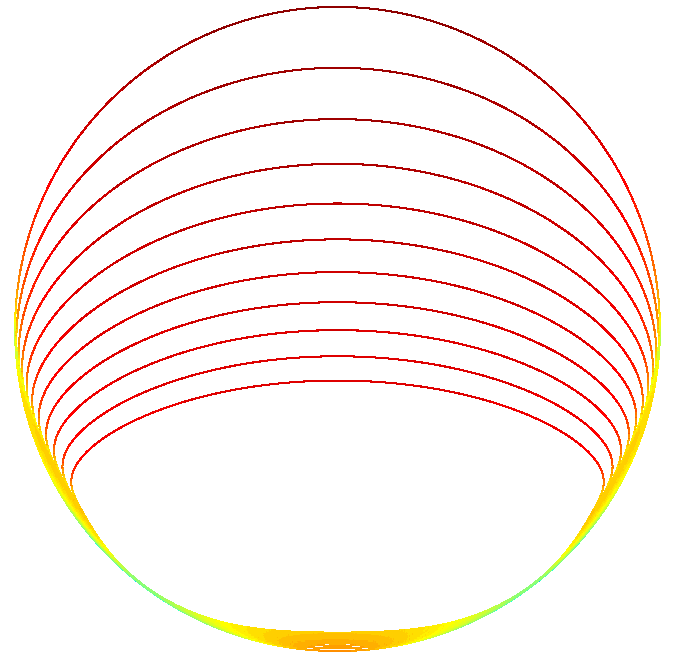
\includegraphics[width = 0.30 \textwidth]{./figs/1b_0d4r1h_shear}
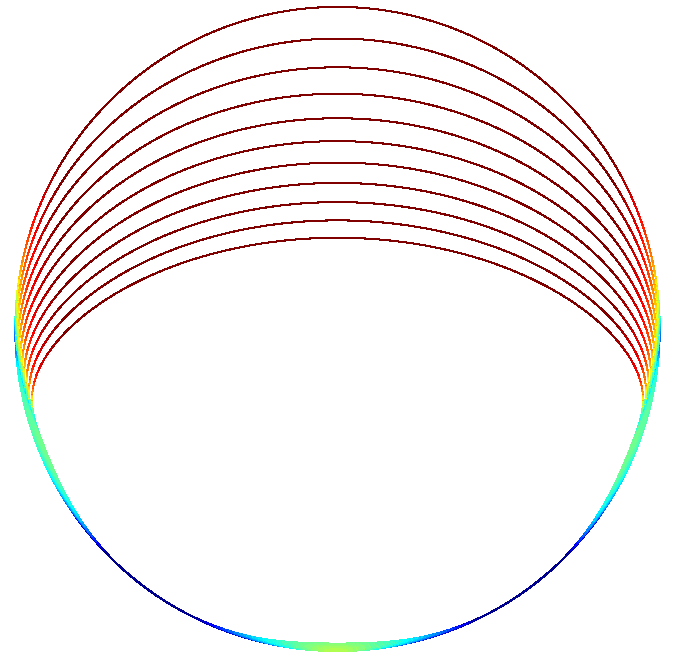
\includegraphics[width = 0.30 \textwidth]{./figs/1b_0d4r0d5h_shear}
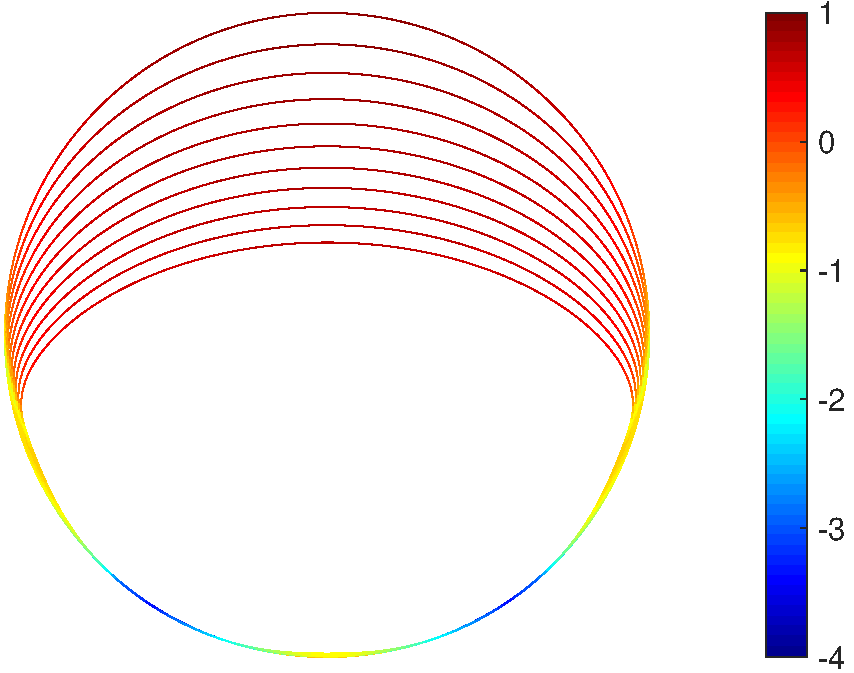
\includegraphics[width = 0.38 \textwidth]{./figs/1b_0d4r0d1h_shear}
\caption{\label{fig:NearWall} 
  A single body eroding in a Stokes flow. The color denotes the
  logarithm of the shear stress on the body. Therefore, erosion is
  fastest in the red regions (top half)and slowest in the blue regions
  (lower half).  The body is initialized at three different distances
  from the lower wall: $d=h$ (left), $h/2$ (middle), and $h/10$
  (right).}
\end{center}
\end{figure}
\begin{figure}[H]
\begin{center}
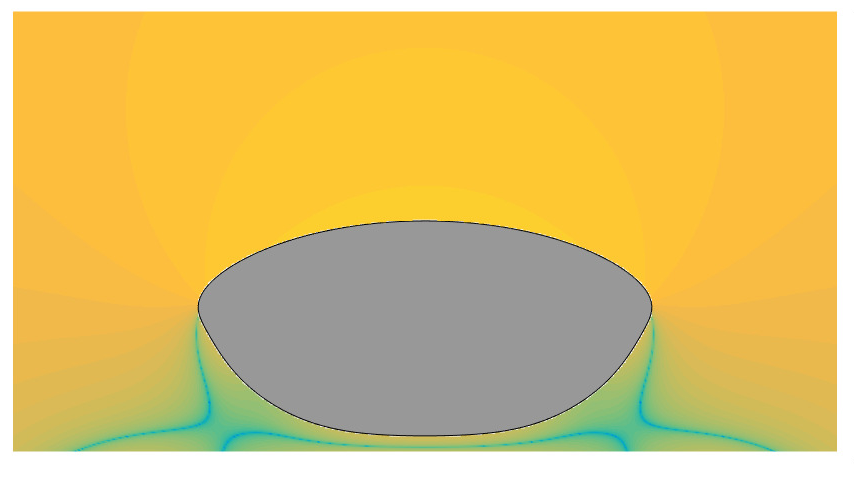
\includegraphics[width = 0.30 \textwidth]{./figs/1b_0d4r1h_vort}
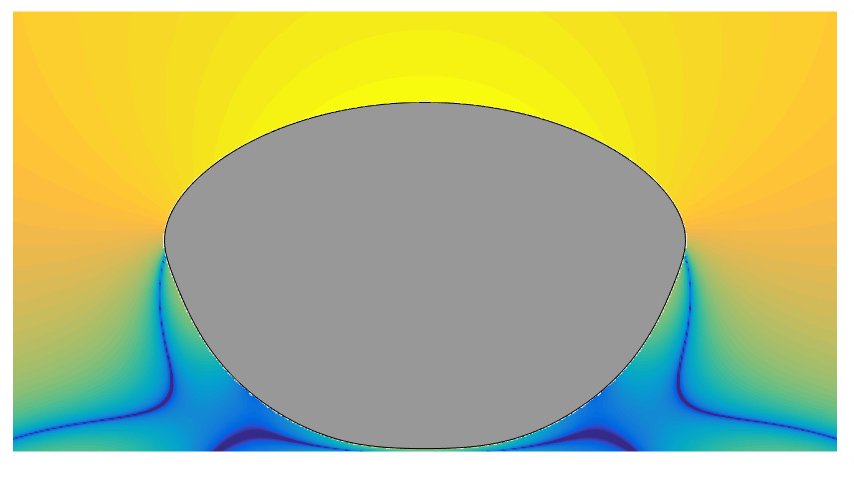
\includegraphics[width = 0.30 \textwidth]{./figs/1b_0d4r0d5h_vort}
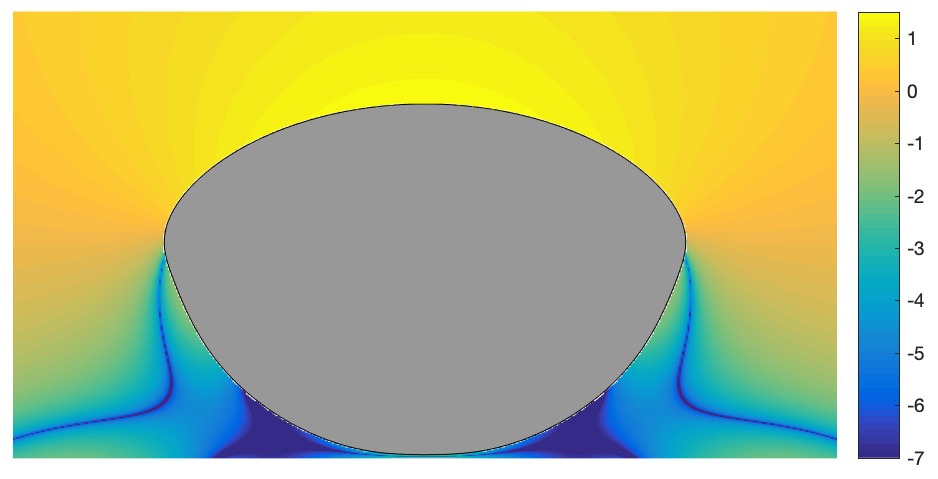
\includegraphics[width = 0.33 \textwidth]{./figs/1b_0d4r0d1h_vort}
\caption{\label{fig:NearWall_vort} The vorticity of the fluid with a single body eroding 
at time t=0.1001. The initial distances from body to wall are $h$ (left), $h/2$
  (middle), and $h/10$ (right).  }
\end{center}
\end{figure}


%%%%%%%%%%%%%%%%%%%%%%%%%%%%%%%%%%%%%%%%%%%%%%%%%%%%%%%%%%%%%%%%%%%%%%%
\subsection{20 Bodies at a Medium Porosity}
%%%%%%%%%%%%%%%%%%%%%%%%%%%%%%%%%%%%%%%%%%%%%%%%%%%%%%%%%%%%%%%%%%%%%%%
We consider 20 eroding bodies that are discretized with $N_\iin=256$
points and are initially placed in $[-1,1] \times [-1,1]$.  The
background flow is the Hagen-Poiseuille flow
\begin{align}
  \UU(\xx)=U \left[
  \begin{array}{c}
    1-y^2 \\ 0
  \end{array}
  \right],
\end{align}
where the flow rate $U$ is chosen so that the pressure drop from $x=-2$
to $x=2$ is held fixed at 2.  We start by analyzing the effect of
erosion on the area fraction and the flow rate.  In
Figure~\ref{fig:Eroding20flowrate}(a), we plot the area fraction as a
function of normalized time.  Initially, 62\% of the geometry is eroded
bodies corresponding to a porosity of $0.38$, and the area fraction
decreases to 0 as the bodies erode.  The trend of the area fraction
resembles that of our previous work~\cite{qua-moo2018} (Figure 10(a)),
but with a larger initial area fraction.  We also compute the flow rate
$U$ required to maintain a constant pressure drop across the channel in
Figure~\ref{fig:Eroding20flowrate}(b).  Again, the trend of $U$
resembles that of our previous work~\cite{qua-moo2018} (Figure 10(b)),
except that the initial flow rate is an order of magnitude smaller
because of the larger initial area fraction.  Starting around normalized
time $0.2$, Figure~\ref{fig:Eroding20flowrate}(b) is roughly linear
which indicates that the flow rate can be written as a power law.  Using
a line of best fit, the flow rate is approximately 
\begin{align} 
  U \approx \left(\frac{t}{t_f}\right)^{3.43},
\end{align}
which is the dashed line in Figure~\ref{fig:Eroding20flowrate}(b).

\begin{figure}[H]
\begin{subfigure}[b]{0.55\textwidth}
\includegraphics*[width =\linewidth]{./figs/porosity20dense}
\caption{}
\end{subfigure}
\begin{subfigure}[b]{0.5\textwidth}
\includegraphics*[width =\linewidth]{./figs/flow_rate20dense}
\caption{}
\end{subfigure}
\caption{\label{fig:Eroding20flowrate}(a): The area fraction of 20
nearly touching eroding bodies versus normalized time. (b): The incoming
flow rate, $U$, for a fixed pressure drop across the channel versus
normalized time.  The flow rate is initially very small, but it
eventually increases as a power law (dashed line) towards the flow rate
$U=1$ that occurs once all the bodies have eroded.}
\end{figure}

Snapshots of the bodies at four equispaced times are shown in
Figure~\ref{fig:Eroding20vort}.  The color is the vorticity which is
equivalent to the shear stress when restricted to the eroding bodies.
Therefore, erosion is fastest in regions where the magnitude of the
vorticity is largest.  Initially, several of the eroding bodies are
closer to the outer wall than the $5h$ threshold required to guarantee
sufficiently accurate quadrature with the trapezoid rule.  In
particular, with $h=L_2/N_\out$, the distance between bodies 1, 6, 13,
and 15 are $1.3h$, $2.9h$, $2.8h$, and $1.3h$, respectively.  In
addition, the distance between several pairs of eroding bodies is too
small to be accurately resolved with the trapezoid rule at the
prescribed resolution.  Particular pairs include bodies 1 \& 6, 3 \& 9,
6 \& 8, and 14 \& 18.  By using the Barycentric quadrature rule, the
interaction between these nearly-touching bodies can be accurately
resolved at the prescribed resolution.

\begin{figure}[H]
\begin{center}
  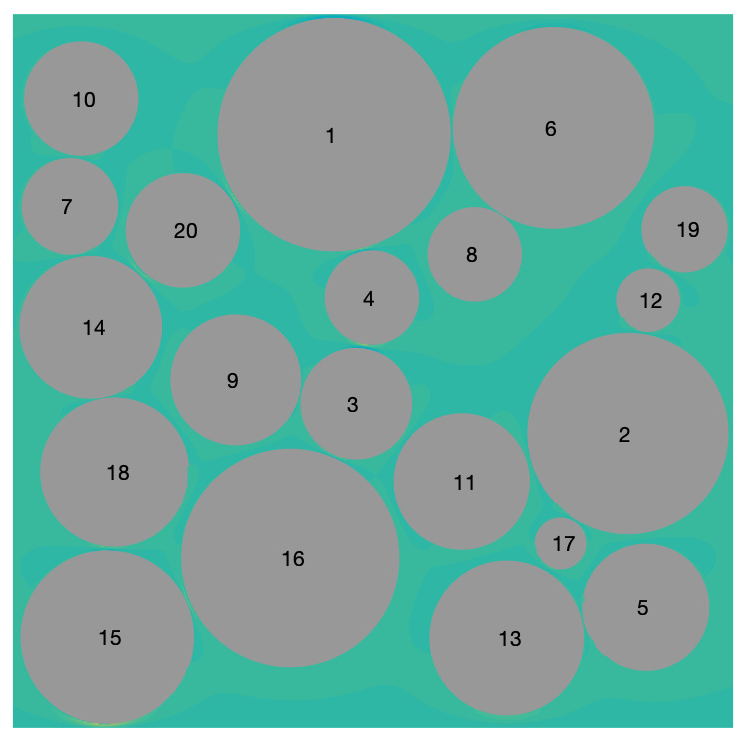
\includegraphics[height=0.225\textwidth]{./figs/20b_dense1}
  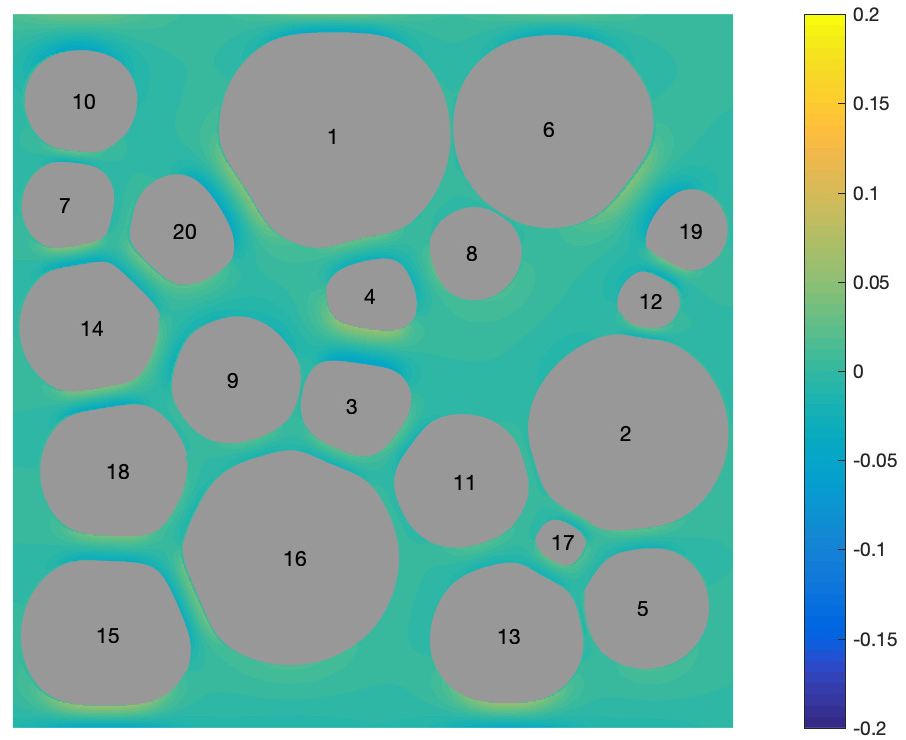
\includegraphics[height=0.225\textwidth]{./figs/20b_dense101}
  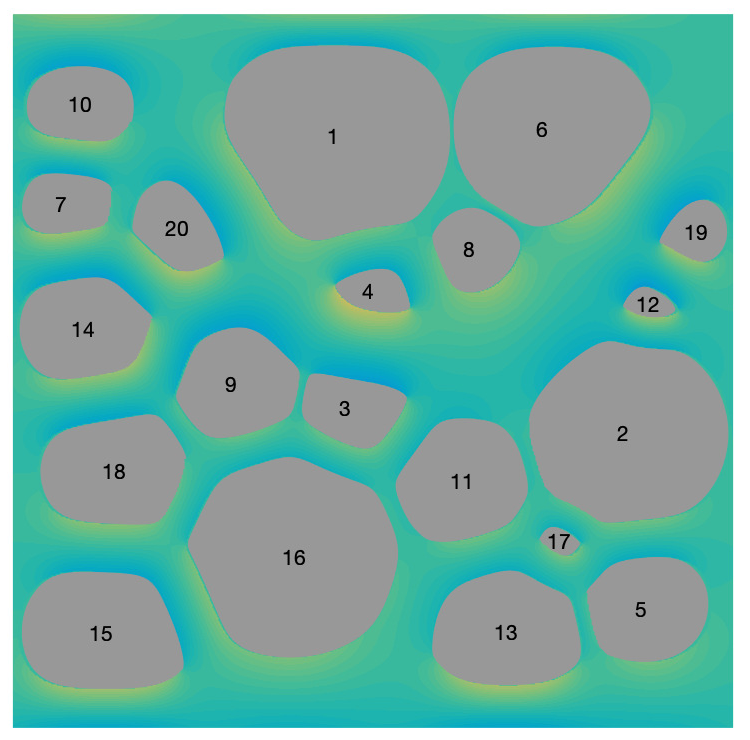
\includegraphics[height=0.225\textwidth]{./figs/20b_dense201}
  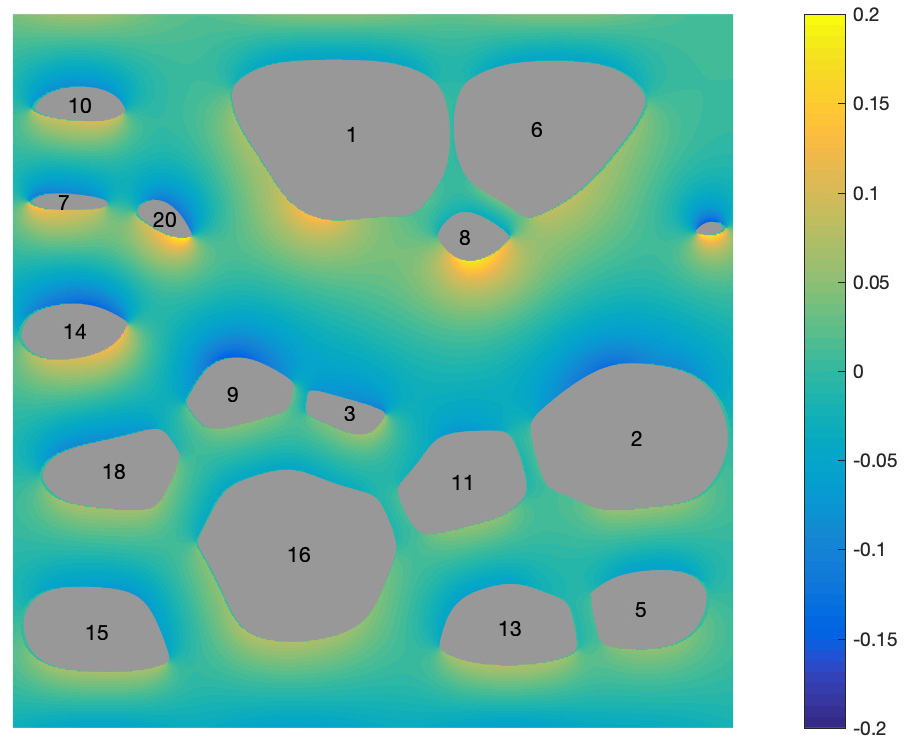
\includegraphics[height=0.225\textwidth]{./figs/20b_dense301}
\caption{\label{fig:Eroding20vort} Erosion of 20 nearly touching bodies
with the fixed pressure drop condition. The color is the vorticity of
the fluid. The four snapshots are evenly spaced in time. We use $N_\iin
= 256$ discretization points on the bodies and $\Dt=10^{-4}$.  In the
forth frame, bodies 4, 12, and 17 have vanished completely, and body 19
has almost completely eroded.}
\end{center}
\end{figure}

In~\cite{qua-moo2018}, we observed that erosion causes the space between
nearly touching bodies to quickly expand, and flat faces develop along
the region of near contact.  This qualitative behavior is present in
Figure~\ref{fig:Eroding20vort} between bodies 3 \& 4, 15 \& 16, and
others.  However, now that we can resolve bodies that are much closer
together, we observe that, at least initially, very little erosion
occurs between certain pairs of bodies.  For instance the opening
between bodies 1 \& 6 grows much slower than the opening between bodies
15 \& 16.  A common feature of the openings that grow slowly is that
they are nearly perpendicular to the main flow direction, and this
results in very low erosion because of the small shearing.  For example,
the openings between the pair of bodies 1 \& 6, 3 \& 9, and 5 \& 13. 

In this example, we also observe that erosion creates a network of
channels from the inlet to outlet where the velocity and vorticity, and
therefore erosion rate, are much larger than in other regions.  These
channels can be further visualized by considering the streamlines.  In
Figure~\ref{fig:Eroding20tracer}, we freeze the geometry at the second
time step from Figure~\ref{fig:Eroding20vort}, and we plot 200
trajectories that are initialized at $x=-1$ and equispaced in $y$.  The
trajectories are shown at 5 different times, and the final plot is a
zoom in of the lower right quadrant of the fifth time step.  There are
three clear regions where the tracers pass through the geometry fastest.
Two of these regions are located between the bodies and the solid walls
at $y=\pm 1$, and the third cuts through the porous region with the
upper part of the channel formed by bodies 1, 4, 6, and 8.  Since the
flow is fastest in these regions, the shearing is largest, and this
causes these openings to grow fastest which can be observed in
Figure~\ref{fig:Eroding20vort}.

\begin{figure}[H]
\begin{center}
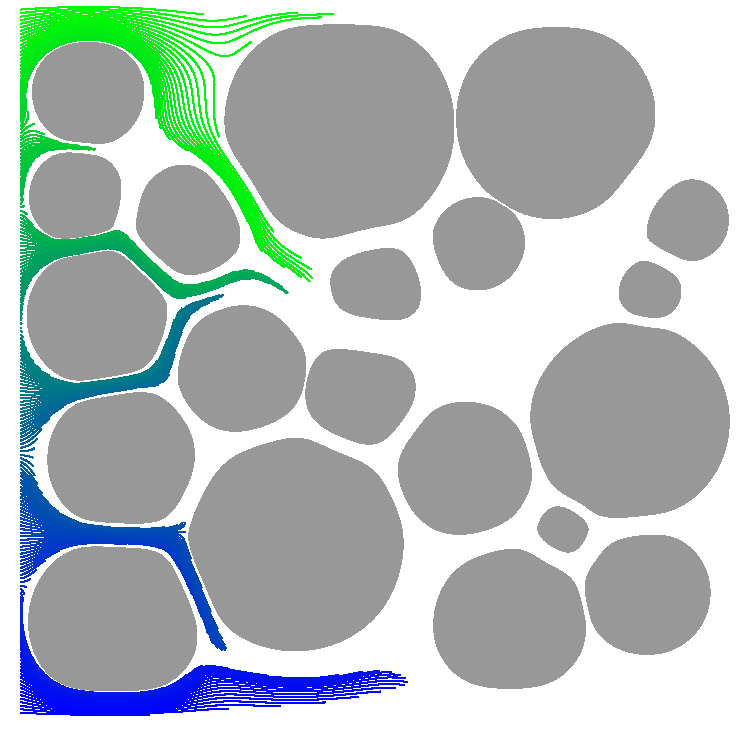
\includegraphics[width = 0.32 \textwidth]{./figs/tracer_20b30}
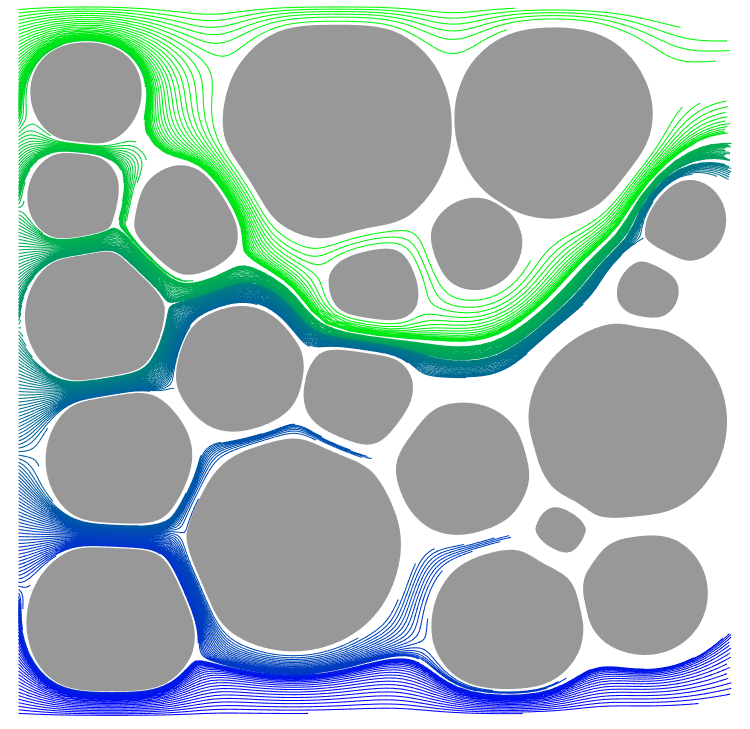
\includegraphics[width = 0.32 \textwidth]{./figs/tracer_20b90}
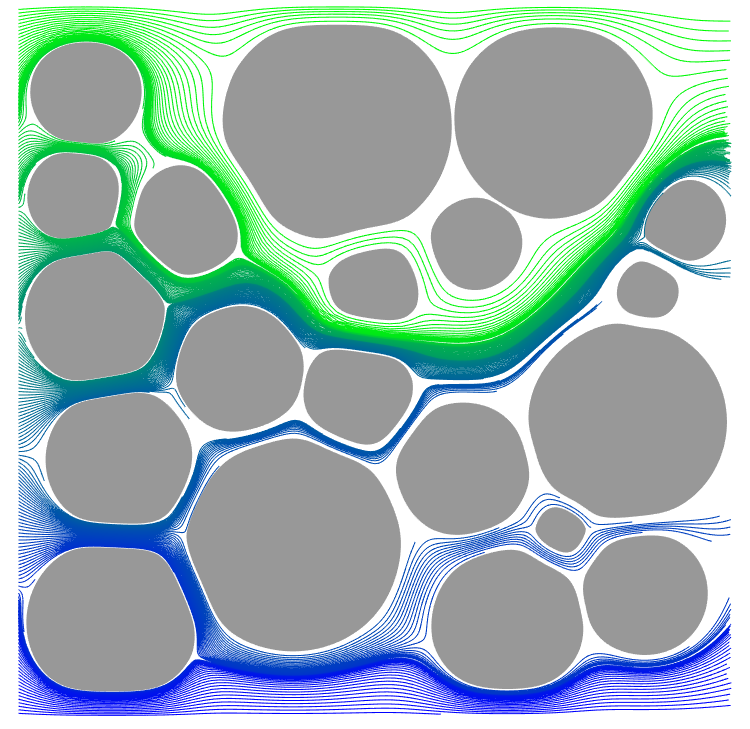
\includegraphics[width = 0.32 \textwidth]{./figs/tracer_20b150}\\
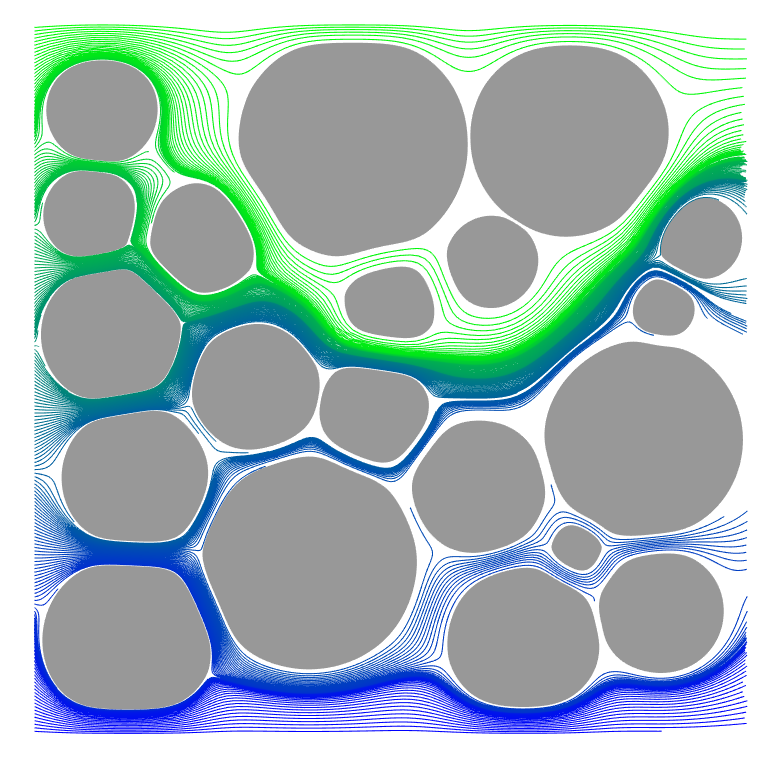
\includegraphics[width = 0.32 \textwidth]{./figs/tracer_20b210}
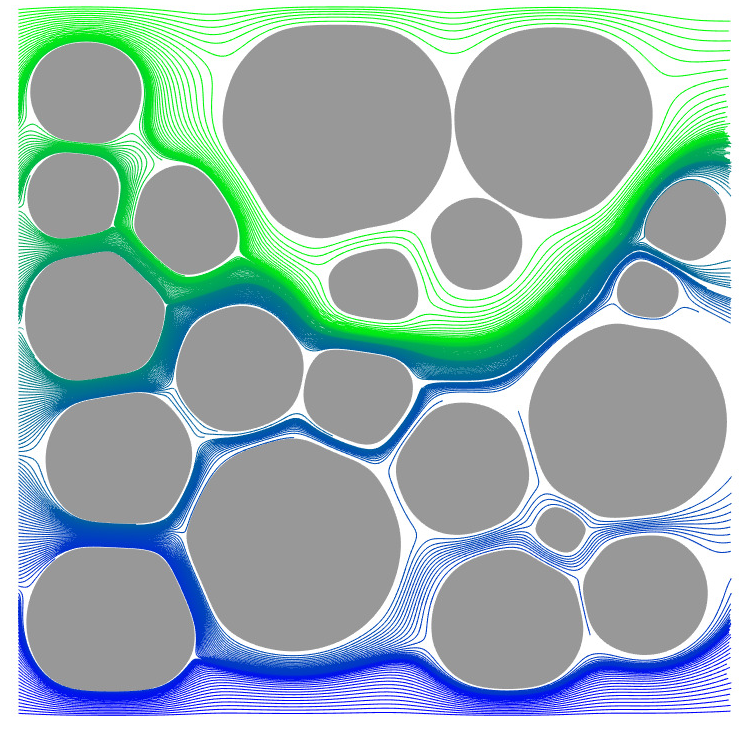
\includegraphics[width = 0.32 \textwidth]{./figs/tracer_20b270}
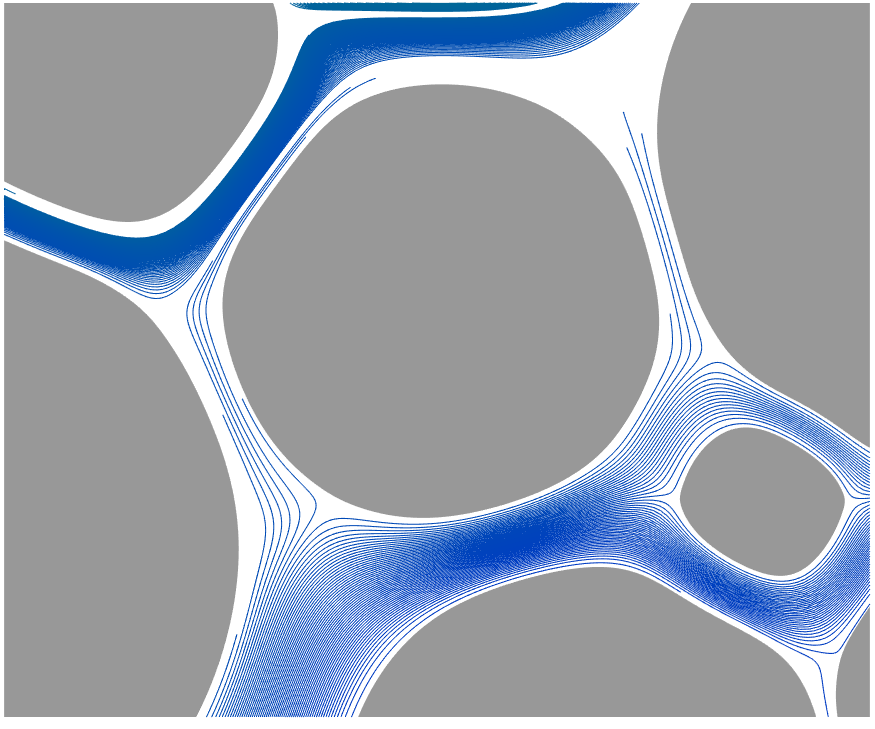
\includegraphics[width = 0.32 \textwidth]{./figs/tracer_20b270_zoom}
\caption{\label{fig:Eroding20tracer}200 trajectories in the second
geometry from Figure~\ref{fig:Eroding20vort}. The trajectories are
initialized at $x=-1$ and are equally spaced in the $y$-direction. The
first five snapshots are evenly spaced in time.  The bottom right frame
is a zoom window of the fifth snapshot.  Since we use a Barycentric
quadrature rule and the fourth-order Runge-Kutta method, the tracers can
be very close to but not penetrate the bodies.}
\end{center}
\end{figure}

Next, we use the tracer trajectories to compute the anomalous diffusion
rates and the tortuosities in the eroding geometry.  Since these
calculations use a statistical analysis of the tracer trajectories, we
increase the number of trajectories to $N_p = 1000$.  Again, the tracers
are initialized at $x=-1$, and their $y$ coordinates are distributed
evenly across the entire channel.  To compute the tortuosity, we
require the velocity at the initialization points of the tracers.  These
normalized velocities are plotted in Figure~ref{fig:Eroding20tort}(a)
for the eroded geometry with porosity 62.9\% (see
Figure~\ref{fig:Eroding20tort}(c)).  The velocities are similar to the
work of Matyka et al.~\cite{matyka2008tortuosity} (see Figure 4(a)),
except that our cross-section does not cut through any of the bodies.
Next, in Figure~\ref{fig:Eroding20tort}(b), we plot the local
tortuosity~\eqref{eqn:localTort} by calculating the length of each
trajectory as it traverses the channel from $x=-1$ to $x=1$ in
Figure~\ref{fig:Eroding20tort}(b), and dividing by the length of the
channel.  The local tortuosity ranges from 1 to 1.27, meaning that one
of the tracers travelled 27\% farther than it would have if the bodies
had been absent.  The average tracer travelled 9.79\% farther than if
the bodies had been absent, meaning that the tortuosity of the eroded
channel is $1.098$.  Again, comparing the local tortuosity to
Matyka~\cite{matyka2008tortuosity} (Figure 4(b)), the results are
qualitatively similar. However, since our initial cross-section does not
cut through any bodies, the local tortuosity does not have any gaps.
The discontinuities correspond to neighboring tracers with one traveling
much farther than the other.  In Figure~\ref{fig:Eroding20tort}(c), we
plot pairs of trajectories that correspond to the ten largest jumps in
the local tortuosity.  Corresponding pairs are always plotted in the
same color.  The discrepancy between the trajectory lengths can be
attributed to the tracers diverging from one another as they approach
opposite sides of a stagnation point in the flow.

\begin{figure}[H]
\begin{subfigure}[b]{0.45\textwidth}
\begin{subfigure}[b]{\textwidth}
\includegraphics*[width =\linewidth]{./figs/velocity_loc20_268}
\caption{}
\end{subfigure}
\begin{subfigure}[b]{\textwidth}
\includegraphics*[width =0.97\linewidth]{./figs/tort_local20_268}
\caption{}
\end{subfigure}
\end{subfigure}
\begin{subfigure}[b]{0.5\textwidth}
\includegraphics*[width =\linewidth]{./figs/tort_diff_top10_268}
\caption{}
\end{subfigure}
\caption{\label{fig:Eroding20tort} The tortuosity of an eroded geometry
with porosity 62.9\%. (a) The x-component of the velocity $u(-1, y)$
normalized by its maximum velocity of $2.98 \times 10^{-3}$. (b) The
local tortuosity $\tau(y)$ on the cross section $x = -1$.  The spatially
averaged tortuosity through the channel is $1.098$.  (c) The
trajectories resulting in the ten largest differences between
neighboring trajectories.  Neighboring trajectories have the same
color.}
\end{figure}

In Figure~\ref{fig:Eroding20tort_all}, we plot the tortuosity as a
function of the porosity from the initial porosity of $0.38$ until all
the bodies have eroded.  The tortuosity is computed with both the length
of the trajectories~\eqref{eqn:tortuosity1} (red marks) and using the
spatial average of the velocity on an Eulerian
grid~\eqref{eqn:tortuosity2}.  The red square corresponds to the
porosity in Figure~\ref{fig:Eroding20tort}(c).  The methods give similar
results with any discrepancy being accounted for by slow regions of
recirculation.  As the bodies erode, this creates wide channels where
trajectories undergo only minor vertical deflections, and this explains
why the tortuosity eventually decreases with porosity.  The increase in
tortuosity for small porosities occurs because in the absence of erosion
(left plot in Figure~\ref{fig:Eroding20vort}), many of the trajectories,
such as those initialized between bodies 15 \& 18, only perform minor
deflections to pass through the narrow regions, albeit, very slowly.
However, as erosion starts to open the channels, the trajectories
deflect into the fast regions, such as the region above body 11, and
this increases the amount of vertical deflection, and therefore the
tortuosity.


\begin{figure}[H]
\center
\includegraphics*[width =0.5\linewidth]{./figs/tort_eulerian}
\caption{\label{fig:Eroding20tort_all} The tortuosity inside of an
eroding geometry initialized with 20 bodies.  The tortuosity is
calculated using the Eulerian method~\eqref{eqn:tortuosity2} (blue dots)
and Lagrangian method~\eqref{eqn:tortuosity1} (red stars).  The red
square correspond to the geometry in Figure~\ref{fig:Eroding20tort}(c).
The dash line is the fitting line $\widehat{T}(\phi)=\phi^{-p}$ as
$p=0.2064$ and the root-mean-square error is $5.9 \times 10^{-3}$.}
\end{figure}



\begin{figure}[H]
%\caption{\label{fig:Eroding20anomalous} The
%mean squared displacement of the tracer trajectories  at several
%different stages of the erosion process.  As the porosity increases, the
%mean squared displacement tends towards $\sigma^2_\lambda(t) \sim t^$
%}
%\includegraphics*[width =0.45\linewidth]{./figs/20b_first_moment}
\center
\includegraphics*[width =0.45\linewidth]{./figs/20b_second_moment_long}
\caption{\label{fig:Eroding20anomalous} The analysis of anomalous
diffusion in 20 nearly touching bodies with respect to initial porosity (37.68\%) and another six porosities
during the eroding. The dashed line correspondes to a porosity of 100\% and the dashed-dotted line is a 
line of best fit with slope 0.5742.}
\end{figure}


%%%%%%%%%%%%%%%%%%%%%%%%%%%%%%%%%%%%%%%%%%%%%%%%%%%%%%%%%%%%%%%%%%%%%%%
\subsection{20 Bodies at a Low Porosity}
%%%%%%%%%%%%%%%%%%%%%%%%%%%%%%%%%%%%%%%%%%%%%%%%%%%%%%%%%%%%%%%%%%%%%%%
We consider a second example with 20 eroding bodies, but with a smaller
initial porosity.  In Figure~\ref{fig:ErodingLow20vort}, we plot the
eroding geometry and porosity at four evenly spaced instances in time.
Again, the color is the vorticity in the bulk whose magnitude is
equivalent to the erosion rate.  Each body is discretized with $N_\iin =
256$, and the smallest distance between two bodies at the initial
condition is ???\todo[inline]{SH: Fill in this number}.  At this
resolution, this corresponds to a spacing of ???$h$ which is much
too small for the trapezoid rule.  By applying the Barycentric
quadrature rule, there is no issue simulating the erosion until all the
bodies have eroded.

\begin{figure}[H]
\begin{center}
  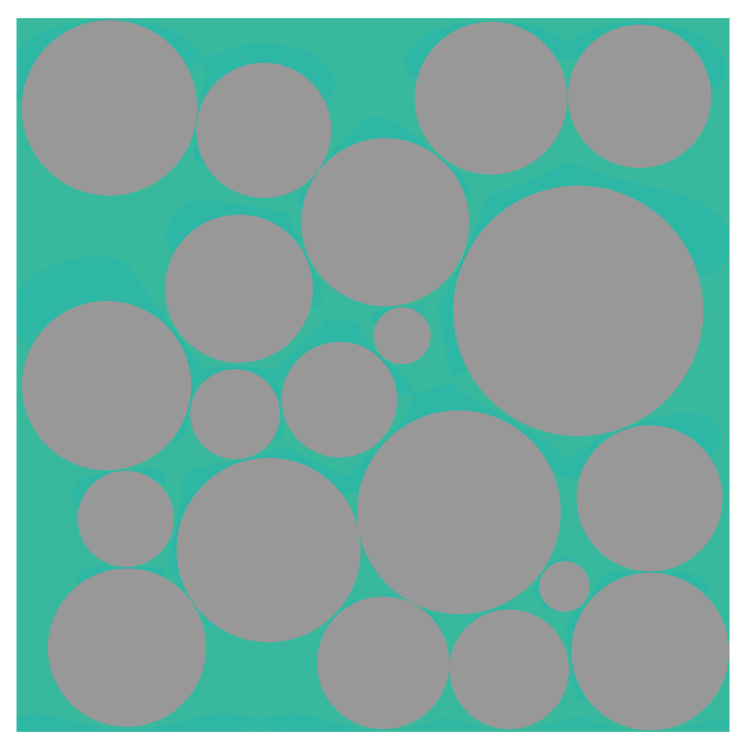
\includegraphics[height=0.225\textwidth]{./figs/20b2_vort1}
  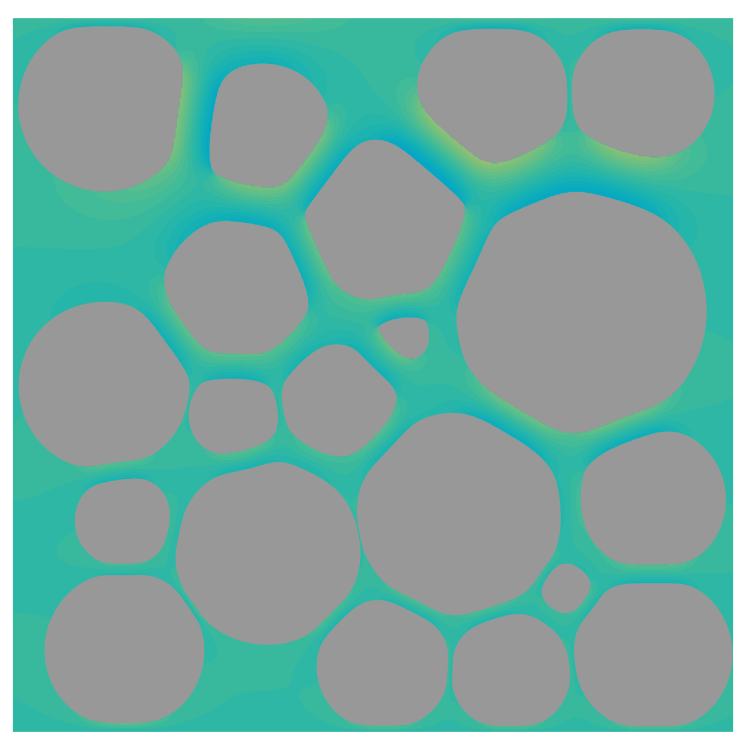
\includegraphics[height=0.225\textwidth]{./figs/20b2_vort150}
  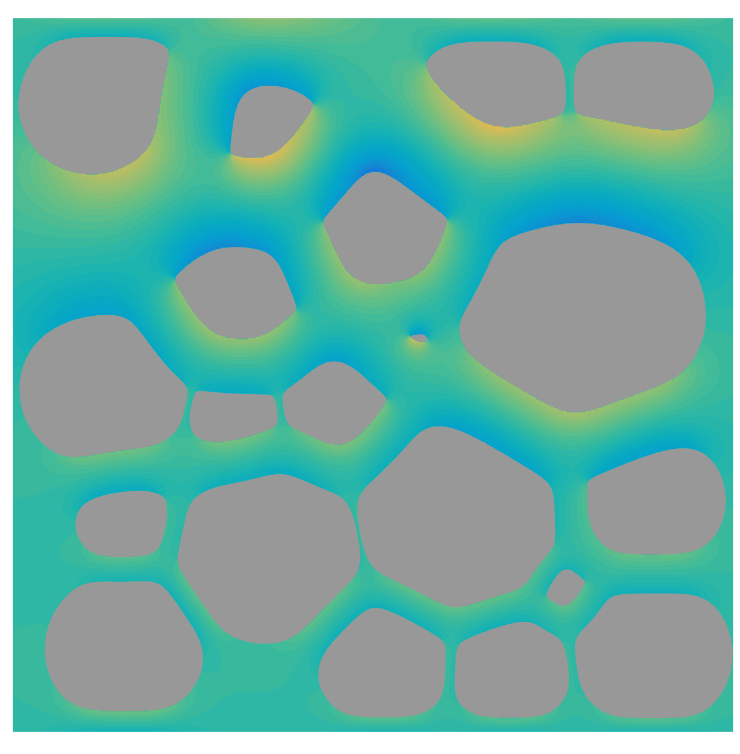
\includegraphics[height=0.225\textwidth]{./figs/20b2_vort300}
  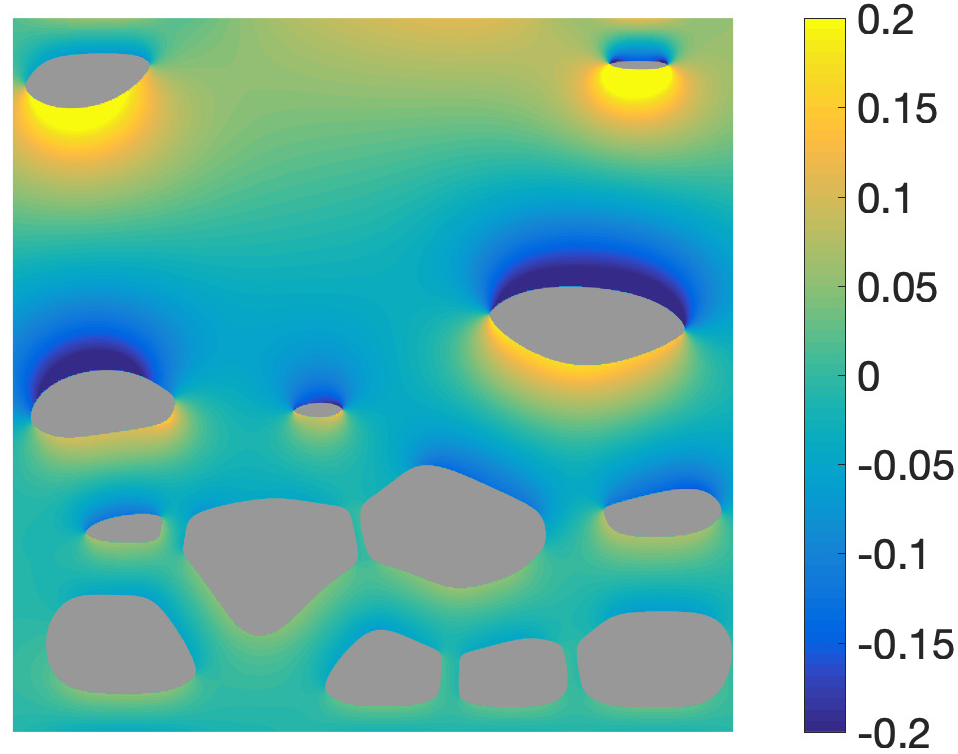
\includegraphics[height=0.225\textwidth]{./figs/20b2_vort450}
\end{center}
\caption{\label{fig:ErodingLow20vort} Erosion of 20 nearly touching
bodies with the fixed pressure drop condition. The color is the
vorticity of the fluid. The 4 snapshots are evenly spaced in time. We
use $N_\iin = 256$ discretization points on the body, a time-step of
$\Dt=10^{-4}$, and smoothing parameters of $\eps= 15/256$ and
$\sigma=10/256 $. }
\end{figure}

We compute the tortuosity using the Eulerian
method~\eqref{eqn:tortuosity2}. In Figure~\ref{fig:ErodingLow20tort}, we
plot the tortuosity with respect to the porosity (blue) and a line of
best fit (black) using the power law $\widehat{T}(\phi) =
\phi^{-p}$~\cite{matyka2008tortuosity}.  This model outperformed the
other three models described in equation~\eqref{eqn:tortuosityModels}.
The root-mean-squared error of the power law is $1.13 \times 10^{-2}$.

Unlike the previous 20 body simulation, the tortuosity decreases
monotonically with the porosity. \todo[inline]{BQ: Why is this the case?
What is special about the last example?}

\begin{figure}[H]
\center
\includegraphics*[width =0.5\linewidth]{./figs/tort_eulerian20b}
\caption{\label{fig:ErodingLow20tort} The tortuosity inside of an
eroding geometry initialized with 20 bodies.  The tortuosity is
calculated using the Eulerian method~\eqref{eqn:tortuosity2} (blue
dots).  The dash line is the fitting line $\widehat{T}(\phi)=\phi^{-p}$
as $p=0.1669$ and the root mean square deviation is $1.13 \times
10^{-2}$.}
\end{figure}



%%%%%%%%%%%%%%%%%%%%%%%%%%%%%%%%%%%%%%%%%%%%%%%%%%%%%%%%%%%%%%%%%%%%%%%
\subsection{50 eroding bodies}
%%%%%%%%%%%%%%%%%%%%%%%%%%%%%%%%%%%%%%%%%%%%%%%%%%%%%%%%%%%%%%%%%%%%%%%
{\color{red}
The second nearly touching bodies case is 50 bodies in a Hagen-Poiseuille flow.
}

%%%%%%%%%%%%%%%%%%%%%%%%%%%%%%%%%%%%%%%%%%%%%%%%%%%%%%%%%%%%%%%%%%%%%%%
\subsection{100 eroding bodies}
%%%%%%%%%%%%%%%%%%%%%%%%%%%%%%%%%%%%%%%%%%%%%%%%%%%%%%%%%%%%%%%%%%%%%%%
As a final example, we consider 100 eroding bodies with an initial
porosity near 55\%.  Snapshots of the configurations and vorticity are
in Figure~\ref{fig:Eroding100vort}.

\begin{figure}[H]
 \begin{subfigure}[b]{0.5\textwidth}
\includegraphics*[width =0.9\linewidth]{./figs/100b_50}
\caption{100 bodies and porosity = 55.54\% at t= 0.005}
\end{subfigure}%
\begin{subfigure}[b]{0.5\textwidth}
\includegraphics*[width =1.1\linewidth]{./figs/100b_100}
\caption{99 bodies and porosity = 62.98\% at t= 0.01}
\end{subfigure}
\begin{subfigure}[b]{0.5\textwidth}
\includegraphics*[width =0.9\linewidth]{./figs/100b_150}
\caption{94 bodies and porosity = 72.22\% at t= 0.015}
\end{subfigure}%
\begin{subfigure}[b]{0.5\textwidth}
\includegraphics*[width =1.1\linewidth]{./figs/100b_200}
\caption{82 bodies and porosity = 83.37\% at t= 0.02}
\end{subfigure}
\caption{\label{fig:Eroding100vort} Erosion of 100 bodies with the
  fixed-pressure-drop condition. The color is the vorticity of fluid. In
  this simulation, we use $N_\iin = 256$ discretization points on the
  body, $N_\out = 1024$ points on the outer wall, a time-step of
  $\Dt=10^{-4}$, and smoothing parameters of $\eps= 15/256$ and
  $\sigma=10/256$.}
\end{figure}

To quantify the tortuosity, we compute the relative velocity
(Figure~\ref{fig:Eroding100tort}(a)) and the local tortuosity
(Figure~\ref{fig:Eroding100tort}(b)) of 1000 tracers placed immediately
to the left of the porous region at $x=-1$.  The porosity at this
instance in time is $62.98\%$ and the maximum velocity at $x=-1$ is
$3.90 \times 10^{-4}$. The initial velocity of the tracers is
qualitatively similar to the 20 body example
(Figure~\ref{fig:Eroding20tort}(a)), except with additional maximum and
minimums because of the additional bodies.  Compared to
Figure~\ref{fig:Eroding20tort}(b), the local tortuosity is much more
discontinuous.  These discontinuities can be explained by examining the
trajectories of tracers in Figure~\ref{fig:Eroding100tort}(c).  Here,
there are many instances of neighboring trajectories that are deflected
apart from one another as they tend to a stagnation point in the flow,
and this results in trajectories with significantly different lengths.
At this instance in time one the tracers travels 25.5\% farther than it
would have if the bodies had been absent, and the average tracer
travelled ???\% farther than it would have if the bodies were absent.
Therefore, at this instance in time, the tortuosity is $1.???$.
\todo[inline]{S-H: Fill in the numbers in this paragraph}

\begin{figure}[H]
\begin{subfigure}[b]{0.45\textwidth}
\begin{subfigure}[b]{\textwidth}
\includegraphics*[width =\linewidth]{./figs/velocity_loc100}
\caption{}
\end{subfigure}
\begin{subfigure}[b]{\textwidth}
\includegraphics*[width =\linewidth]{./figs/tort_local100}
\caption{}
\end{subfigure}
\end{subfigure}
\begin{subfigure}[b]{0.5\textwidth}
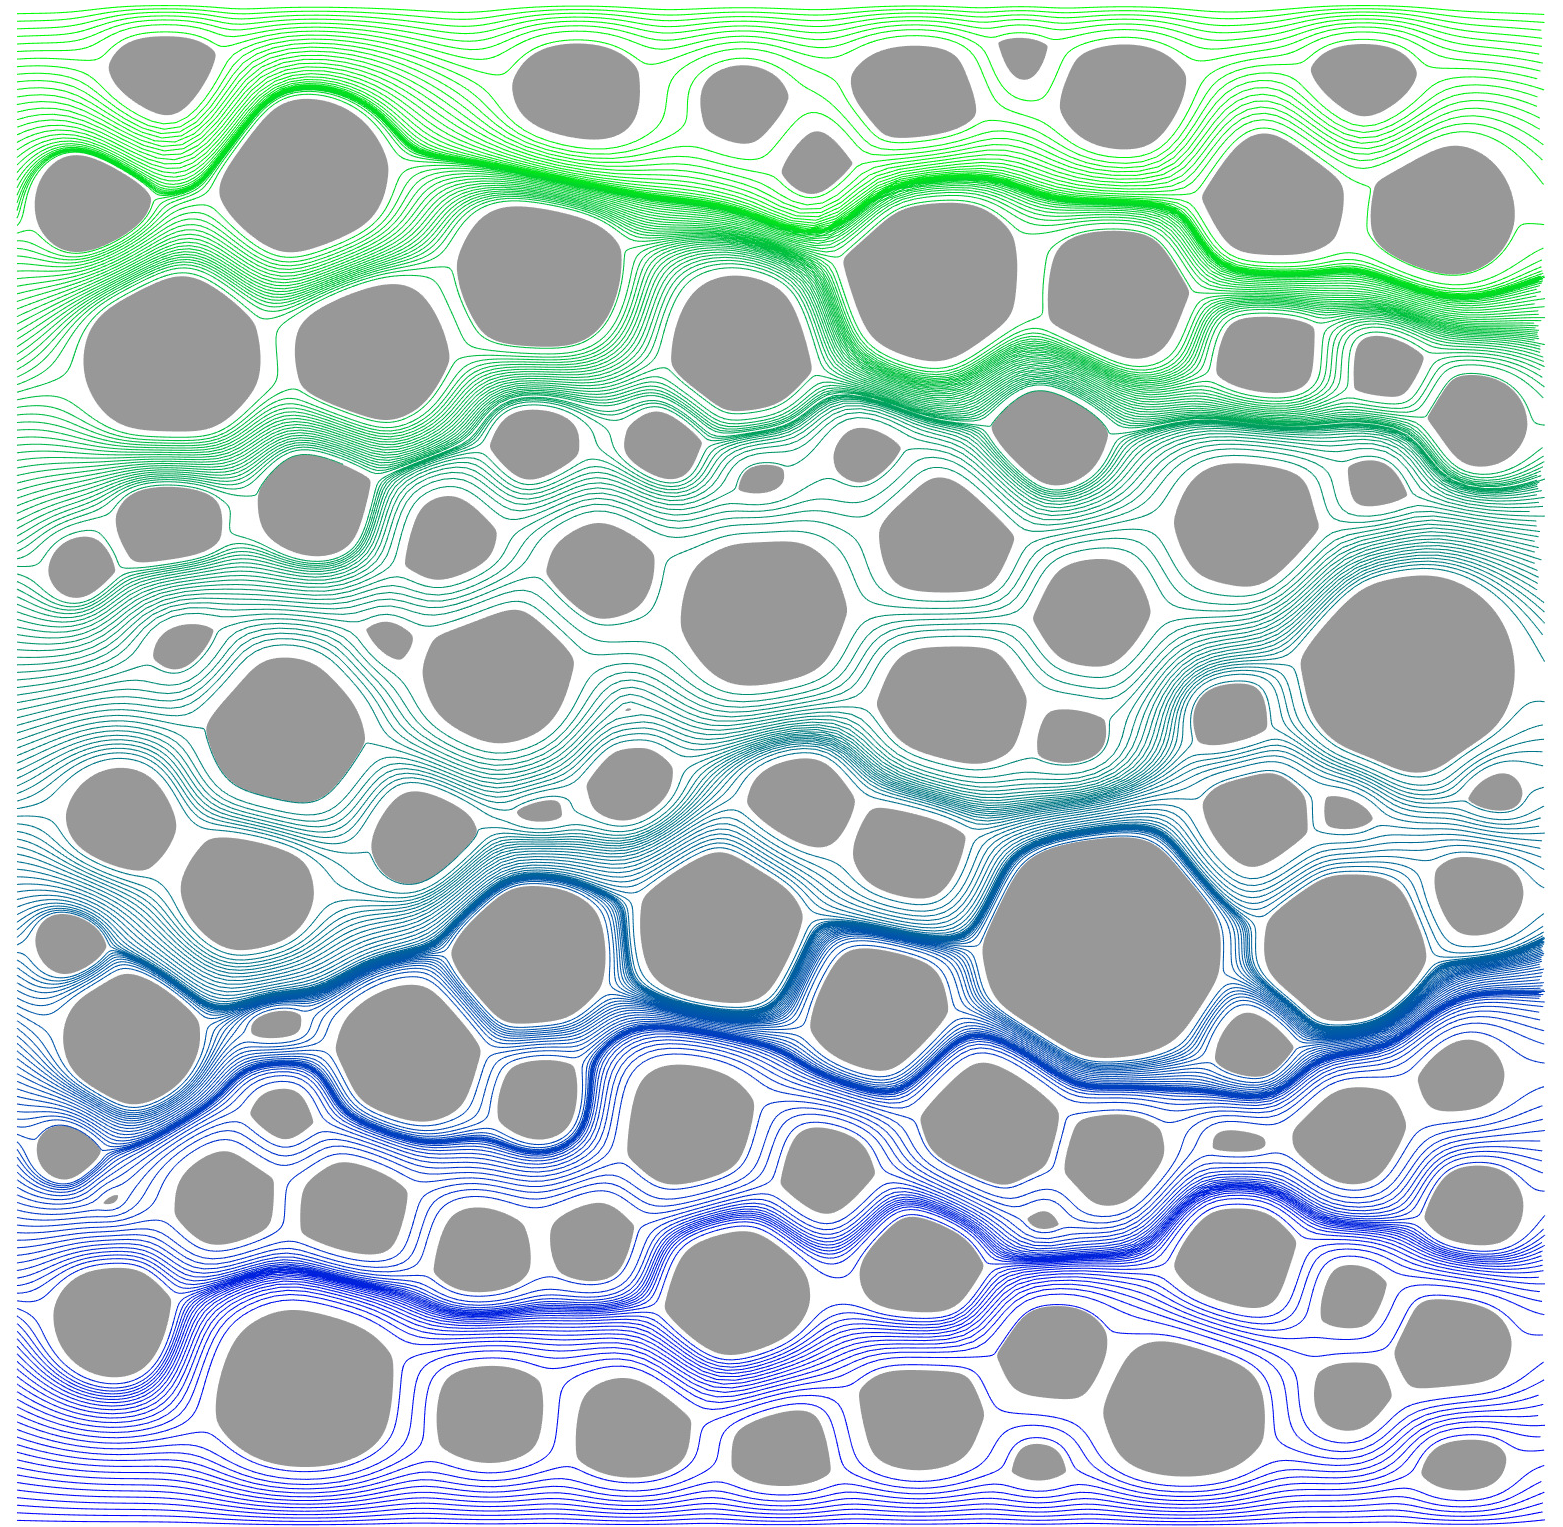
\includegraphics[width = \textwidth]{./figs/100b_t100tracer}
\caption{}
\end{subfigure}
\caption{\label{fig:Eroding100tort} The tortuosity study in the fluid
with 100 bodies when the porosity is 62.98\%.  (a) The x-component
velocity u(-1, y) with respect to its maximum velocity $u_{max}=3.9021
\times 10^{-4}$ at equal spreading tracers on the cross section x = -1.
(b) The local tortuosity $\tau(y)$ on the cross section x = -1. (c) The
trajectories of 200 tracers released at $x = -1$ in the fluid with
multiple bodies.}
\end{figure}

The tortuosity at all porosities from the initial condition until all
the bodies have eroded is in Figure~\ref{fig:Eroding100tort_all}.  The
initial tortuosity is around $T=1.2$ and decays towards $T=1$.  The
tortuosities indicated by the blue dots are calculated using the
Eulerian approach~\eqref{eqn:tortuosity2}, while the red marks use the
Lagrangian approach~\eqref{eqn:tortuosity1}.  Again, the two methods
give comparable results indicating that any recirculation is small and
negligible.  As in the previous examples, the tortuosity depends on the
porosity through a power law model with a small root-mean-squared error
of $5.2 \times 10^{-3}$.  For this example, the logarithm tortuosity
model $\hat{T}(\phi) = 1 - p \ln(\phi)$ achieves a similar
root-mean-squared error.  The tortuosity has one interesting feature
near the end of the simulation where it suddenly increases.  This
behavior can be explained by ... \todo[inline]{S-H: Show me what is
going on here as we discussed.} 

\begin{figure}[H]
\center
\includegraphics*[width =0.5\linewidth]{./figs/tort_eulerian100}
\caption{\label{fig:Eroding100tort_all} The Eulerian and Lagrangian
approach of tortuosity.  The blue dots are Eulerian approach of
tortuosity and the red stars and square are Lagrangian approach of
tortuosity.  The dash line is the fitting line
$\widehat{T}(\phi)=\phi^{-p}$ as $p=0.2459$ and the root-mean-square
error is $5.5 \times 10^{-3}$.  We note that the model
$\widehat{T}(\phi) = 1-p\ln(\phi)$, with $p=0.2631$ has a comparable
root-mean-square error of $5.2 \times 10^{-3}$.}
\end{figure}




Next, we use the 1000 tracer trajectories to compute the first
(Figure~\ref{fig:Eroding100anomalous}(a)) and second
(Figure~\ref{fig:Eroding100anomalous}(b)) moments of the streamlines at
various porosities.  At high porosities, the first moment is similar to
the first-moment of trajectories in a empty channel (black dashed line).
At smaller porosities, the first moment is always linear, but larger
slopes indicate that the length of the trajectories are longer at lower
porosities \todo[inline]{Don't understand how this is the case}.  The
onset of anomalous diffusion is observed in
Figure~\ref{fig:Eroding100anomalous}(b). At early times, the particle
spreading is comparable to that of an open channel (dashed curve)
corresponding to the ballistic regime.  However, as the trajectories
traverse the geometry, a transition to a sub-diffusion case, especially
at low porosities, is evident.  The dashed-dotted line corresponds has a
slope less than 1 indicating the long time behavior of the trajectories
\begin{align*}
  \sigma_\lambda \sim t^{0.8715}.
\end{align*}

\begin{figure}[H]
\center
\includegraphics*[width =0.45\linewidth]{./figs/100b_first_moment}
\includegraphics*[width =0.45\linewidth]{./figs/100b_second_moment}
\caption{\label{fig:Eroding100anomalous} The first and second moments of
trajectories passing through an eroding geometry at several porosities.
The dashed black line corresponds to a porosity of 100\%, and the
dashed-dotted line is a line of best fit with slope 0.8715.}
\end{figure}

Finally, using network models for flow in porous media~\cite{}, the
anomalous diffusion rate can be linked to channel widths between solid
bodies.  We construct a Delaunay triangulation with the centers of the
eroding bodies corresponding to the vertices of the triangles.  Then, if
the side of a triangle connects two vertices, we call the bodies
neighbors.  Then, for each pair of neighbors, we measure the distance
between the bodies.  Once a Delaunay triangulation is formed, it is used
for all subsequent time steps until a body completely disappears.  At
this point, a new Delaunay triangulation is formed.  

We plot the distribution of the gap sizes at four equally spaced points
in time in Figure~\ref{fig:Eroding100gap}.  At the initial configuration, there
are 100 bodies and 318 pairs of neighbors.  The mean distance between
these neighbors is $???  \times 10^{-???}$ and the variance is $???
\times 10^{???}$.  As the bodies erode, the mean and variance of the
distance between the bodies increases.  Finally, at the final time step,
there are only 82 bodies and 254 pairs of neighbors.
\begin{figure}[H]
\begin{subfigure}[b]{0.5\textwidth}
\includegraphics*[width =\linewidth]{./figs/gap_hist100_50}
\caption{100 bodies with 318 gaps at t= 0.005}
\end{subfigure}%
\begin{subfigure}[b]{0.5\textwidth}
\includegraphics*[width =\linewidth]{./figs/gap_hist100_100}
\caption{99 bodies with 312 gaps at t= 0.01}
\end{subfigure}
\begin{subfigure}[b]{0.5\textwidth}
\includegraphics*[width =\linewidth]{./figs/gap_hist100_150}
\caption{94 bodies with 294 gaps at t= 0.015}
\end{subfigure}%
\begin{subfigure}[b]{0.5\textwidth}
\includegraphics*[width =\linewidth]{./figs/gap_hist100_200}
\caption{82 bodies with 254 gaps at t= 0.02}
\end{subfigure}
\caption{\label{fig:Eroding100gap} The distribution of the gaps in the
case of erosion of 100 bodies at four time steps.}
\end{figure}







%\begin{figure}[H]
%\begin{center}
%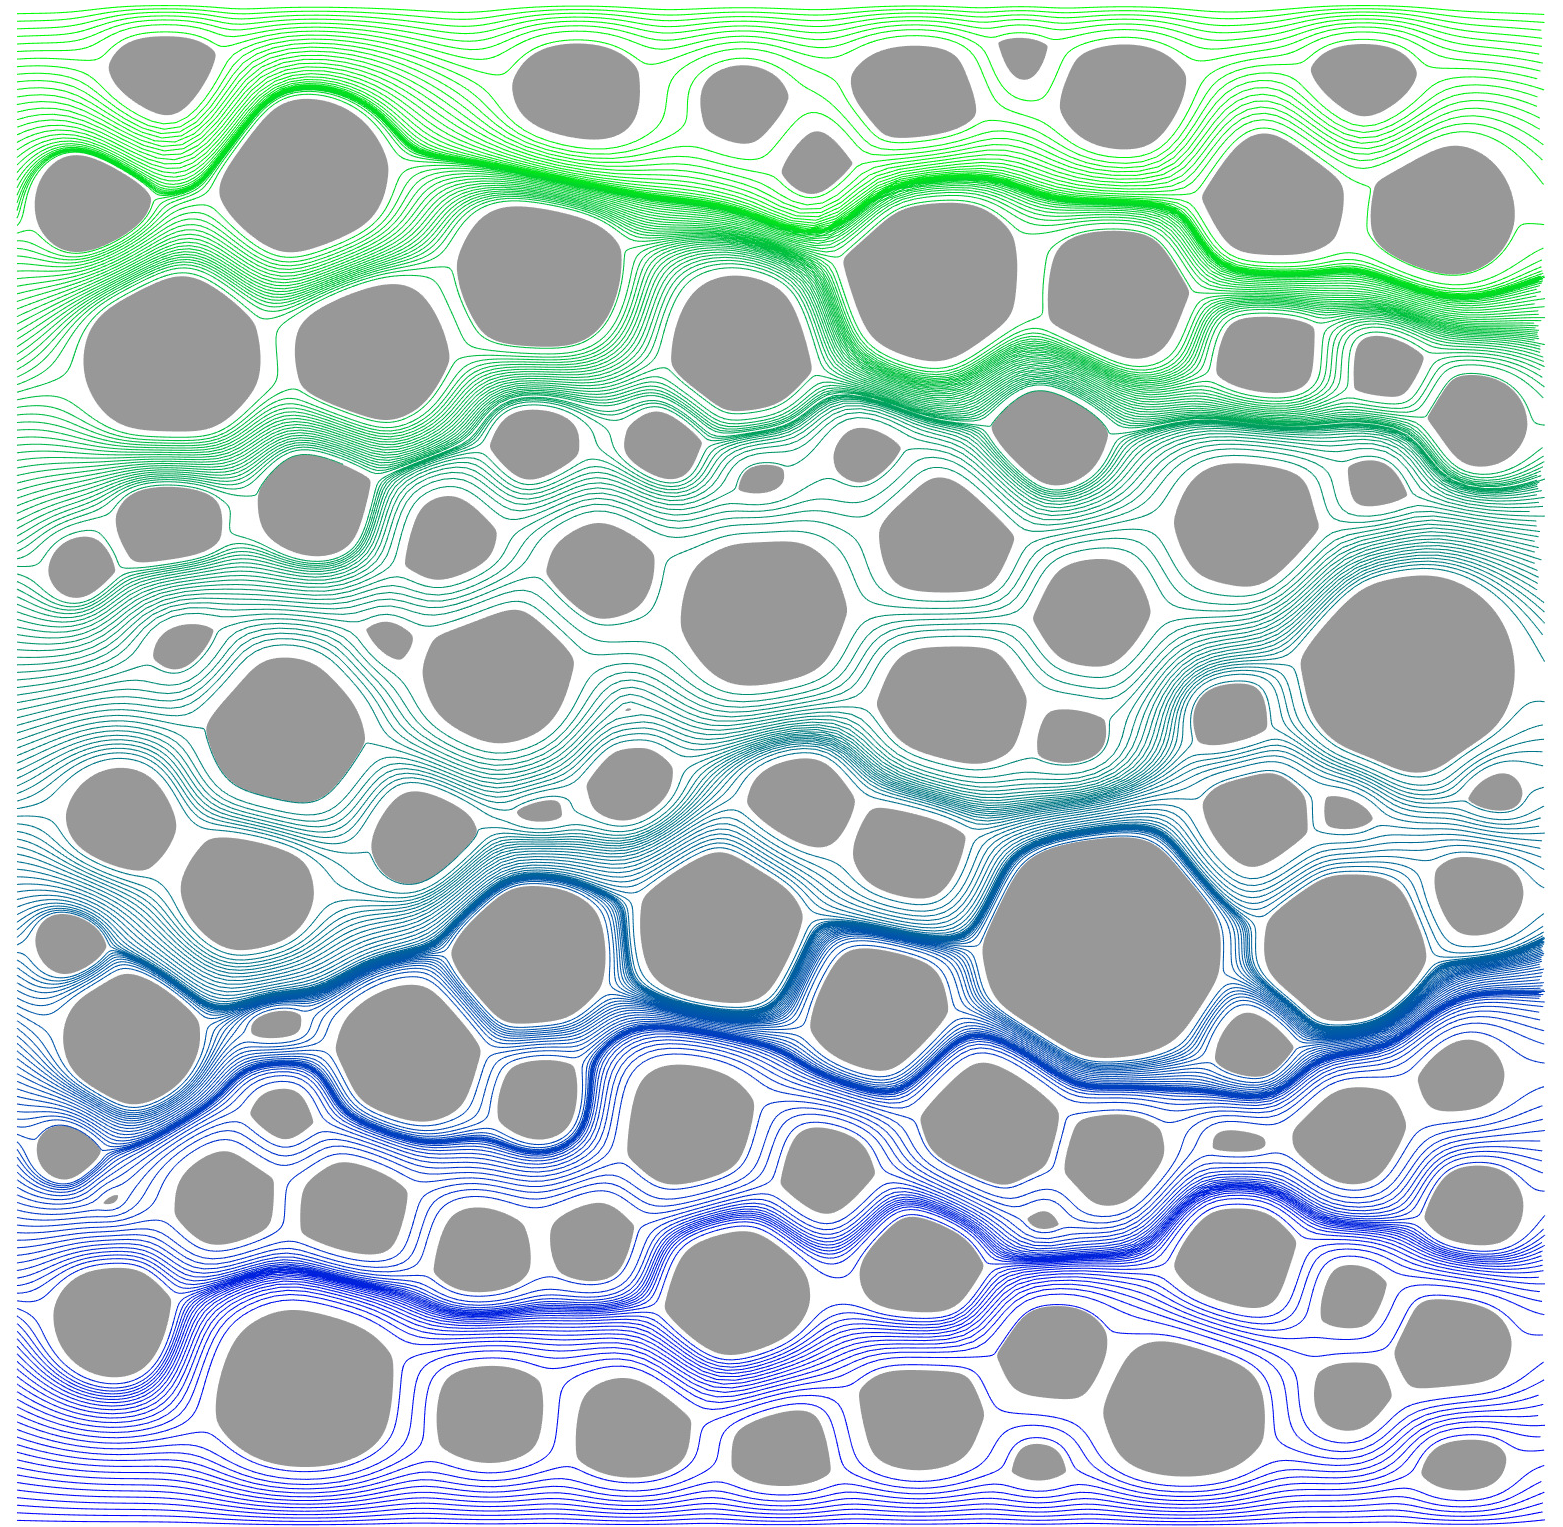
\includegraphics[width = 0.8\textwidth]{./figs/100b_t100tracer}
%\caption{\label{fig:Eroding100tracer} The historical trajectories of 
%200 tracers released at x = -1 in the fluid with multiple bodies.}
%\end{center}
%\end{figure}


%\begin{figure}[H]
%\center
%\includegraphics*[width =0.5\linewidth]{./figs/tort100b_diff_top50}
%\caption{\label{fig:Eroding100tort_traj} The largest 50 difference of 
%local tortuosity $\tau$ at two neighboring tracers in
%100 bodies eroding when the porosity is 62.98 \%
%and the tortuosity is 1.1182. The same color of a pair of trajectories 
%means they are from two neighboring tracers.}
%\end{figure}

%%%%%%%%%%%%%%%%%%%%%%%%%%%%%%%%%%%%%%%%%%%%%%%%%%%%%%%%%%%%%%%%%%%%%%%
\section{Conclusions}
\label{sec:conclusions}
%%%%%%%%%%%%%%%%%%%%%%%%%%%%%%%%%%%%%%%%%%%%%%%%%%%%%%%%%%%%%%%%%%%%%%%


%%%%%%%%%%%%%%%%%%%%%%%%%%%%%%%%%%%%%%%%%%%%%%%%%%%%%%%%%%%%%%%%%%%%%%%
\paragraph{\bf Acknowledgments} BQ and NM were supported by Florida
State University startup funds and Simons Foundation Mathematics and
Physical Sciences-Collaboration Grants for Mathematicians.

\bibliographystyle{plainnat} 
\biboptions{sort&compress}
\bibliography{refs}










%old stuff%
%%%%%%%%%%%%%%%%%%%%%%%%%%%%%%%%%%%%%%%%%%%%%%%%%%%%%%%%%%%%%%%%%%%%%%%%
%\subsection{boundary integral equation formulation} 
%\label{sec:bies}
%add an introduction why we do not use the double-layer potentials of stokes equations but the double-layer potentials of laplace equations to solve stokes equation when we use barycentric approach (or complex variable approach).
%
%\subsubsection{laplace's equations from $\rdb^2$ to $\cdb$ }
%
%let $\omega$ be the domain of fluid. the boundary of $\omega$ is $\gamma$ and the outward normal vector on $\gamma$ is ${\bf n_y}=(n_1,n_2)$.
%
%consider a laplace's equations with dirichlet boundary condition
%\begin{equation}\label{laplace}
%  \begin{cases}
%    \delta {\bf u}=0, & \text{in}\,\,\, \omega \in \rdb^2;\\
%    {\bf u}={\bf f}, & \text{on}\,\,\, \gamma.
%  \end{cases}
%\end{equation}
%
%Let ${\bf x}=(x_1,x_2), {\bf y}=(y_1,y_2)$. Then we have ${\bf r}={\bf x} - {\bf y}$ and $\rho=|\bf r|$.
%The double-layer potential which solves \eqref{Laplace} is 
%\begin{align*}
%\D[\sigma]({\bf x})&=\frac{1}{2\pi}\displaystyle\int_{\Gamma} \frac{{\bf r} \cdot {\bf n_y}}{\rho^2}\sigma({\bf y})ds_y,
%%\frac{1}{2\pi}\displaystyle\int_{\Gamma}\frac{\partial}{\partial {\bf n_y}} \log |{\bf x}-{\bf y}| \sigma({\bf y})ds_y,\\ \\
%%&=\frac{-1}{2\pi}\int_{\Gamma}\frac{{\bf r}\cdot{\bf n_y}}{\rho^2} \sigma({\bf y})ds_y\\ \\
%%&=\frac{-1}{2\pi}\int_{\Gamma}\frac{n_1(x_1-y_1)+n_2(x_2-y_2)}{(x_1-y_1)^2+(x_2-y_2)^2} \sigma({\bf y})ds_y 
%\numberthis\label{DLP:real}
%\end{align*}
%where $\sigma$ is the density function on the boundary $\Gamma$.
%
%
%Consider a Cauchy integral 
%\begin{equation}\label{CI}
%v({x})=\frac{1}{2\pi i}\int_{\Gamma}\frac{\sigma({ y})}{{ y}-{ x}} d{ y},\,\,\,\,\,\,\,\,\, \forall { x} \in \Cdb\setminus \Gamma.
%\end{equation}
%where ${ x}=x_1+ix_2$, $ { y}=y_1+iy_2$, ${ n_y}=n_1+i n_2$ and $d{ y}=i {n_y}ds_y$. It can be shown that 
%the real part of the Cauchy integral in \eqref{CI} is equivalent to the double-layer potential in \eqref{DLP:real}. 
%
%
%\subsubsection{From Stokes DLP to Laplace DLPs}
%
%Let ${\bf x}=(x_1,x_2), {\bf y}=(y_1,y_2)$. Then we have ${\bf r}={\bf x} - {\bf y}$ and $\rho=|\bf r|$.
%
%
%The Stokes double-layer potential  is
%\begin{equation}\label{StokesDLP1}
%\D[\boldsymbol\sigma]({\bf x}):=\frac{1}{\pi}\int_{\Gamma}\left(\frac{{\bf r} \cdot {\bf n_y}}{\rho^2}\frac{{\bf r} \otimes {\bf r}}{\rho^2}\right) {\boldsymbol\sigma({\bf y})} d s_y.
%\end{equation}
%We could rewrite the Stokes DLP in terms of the Laplace DLP as
%\begin{align*}\label{StokesDLP2}
%\D[\boldsymbol\sigma]({\bf x})=\frac{1}{2\pi}\int_{\Gamma}&\frac{{\bf n_y}}{\rho^2}({\bf r} \cdot {\boldsymbol \sigma})ds_y+\frac{1}{2\pi}\nabla\int_{\Gamma}\frac{{\bf r} \cdot {\bf n_y}}{\rho^2}({\bf y} \cdot{\boldsymbol \sigma})ds_y\\
%&-\frac{1}{2\pi}x_1 \nabla\int_{\Gamma}\frac{{\bf r} \cdot {\bf n_y}}{\rho^2}\sigma_1ds_y-\frac{1}{2\pi}x_2\nabla\int_{\Gamma}\frac{{\bf r} \cdot {\bf n_y}}{\rho^2}\sigma_2ds_y. \numberthis
%\end{align*}
%

 
%%%%%%%%%%%%%%%%%%%%%%%%%%%%%%%%%%%%%%%%%%%%%%%%%%%%%%%%%%%%%%%%%%%%%%%%
%\subsection{Computing the shear stress}
%\label{sec:shearStressLP}
%
%To calculate the shear stress, we need to know the gradient of double-layer potential in \eqref{StokesDLP2} 
%\begin{align*}\label{SSLP}
%\nabla\D[\boldsymbol\sigma]({\bf x})=\frac{1}{2\pi}\nabla\int_{\Gamma}&\frac{{\bf n_y}}{\rho^2}({\bf r} \cdot {\boldsymbol \sigma})ds_y+\frac{1}{2\pi}\nabla^2\int_{\Gamma}\frac{{\bf r} \cdot {\bf n_y}}{\rho^2}({\bf y} \cdot{\boldsymbol \sigma})ds_y\\
%&-\frac{1}{2\pi}\nabla\left(x_1 \nabla\int_{\Gamma}\frac{{\bf r} \cdot {\bf n_y}}{\rho^2}\sigma_1ds_y\right)-\frac{1}{2\pi}\nabla\left(x_2\nabla\int_{\Gamma}\frac{{\bf r} \cdot {\bf n_y}}{\rho^2}\sigma_2ds_y\right). \numberthis
%\end{align*}
%
%
%
%
%%%%%%%%%%%%%%%%%%%%%%%%%%%%%%%%%%%%%%%%%%%%%%%%%%%%%%%%%%%%%%%%%%%%%%%%
%\subsection{Boundary evolution in the {\thL} framework} 
%\label{sec:thetaL}
%
%
%%%%%%%%%%%%%%%%%%%%%%%%%%%%%%%%%%%%%%%%%%%%%%%%%%%%%%%%%%%%%%%%%%%%%%%%
%\subsection{Solving the BIE}
%\label{sec:BIE}
%\subsubsection{Interior Case}
%Consider a Cauchy integral 
%\begin{align}\label{CIFI}
%\frac{1}{2\pi i}\int_{\Gamma}\frac{v^-({ y})}{{ y}-{ x}} d{ y}
%&=\begin{cases}
%\,v(x), &{ x} \in \Omega,\\ 
%\,0,  &{ x} \in \Cdb\setminus \bar{\Omega}.
%\end{cases}
%\end{align}
%By the identity of Cauchy Integral Formula $\displaystyle\frac{1}{2 \pi i}\int_{\Gamma}\frac{1}{{ y}-{ x}} d{ y}=1,$ we can rewrtie \eqref{CIFI} and get 
%\begin{equation}
%\frac{1}{2\pi i}\int_{\Gamma}\frac{v^-({ y})-v(x)}{{ y}-{ x}} d{ y}=0,\,\,\,\,\,\,\,\,\, \forall { x} \in \Omega.
%\end{equation}
%\begin{equation}\label{dNCI}
%v'({x})=\frac{1}{2\pi i}\int_{\Gamma}\frac{v^-({ y})}{(y- x)^2} d{ y},\,\,\,\,\,\,\,\,\, \forall { x} \in \Omega.
%\end{equation}
%By the identity of Cauchy Integral Formula $\displaystyle\frac{1}{2 \pi i}\int_{\Gamma}\frac{1}{( y- x)^n} d{ y}=0$ for integer n $\neq 1$, we can rewrtie \eqref{dNCI} and get 
%\begin{equation}
%\frac{1}{2\pi i}\int_{\Gamma}\frac{v^-({ y})-v(x)-(y-x)v'(x)}{(y-x)^2} d{ y}=0,\,\,\,\,\,\,\,\,\, \forall { x} \in \Omega.
%\end{equation}
%
%\subsubsection{Exterior case}
%Consider a Cauchy integral formula for the exterior domain
%\begin{align}\label{CIFE}
%\frac{1}{2\pi i}\int_{\Gamma}\frac{v^+({ y})}{{ y}-{ x}} d{ y}
%&=\begin{cases}
%\,v_{\infty}, &{ x} \in \Omega,\\ 
%\,-v(x)+v_{\infty},  &{ x} \in \Omega^c,
%\end{cases}
%\end{align}
%where $v_{\infty}=\displaystyle\lim_{x \to \infty}v(x)$.
%\begin{equation}
%\frac{1}{x-a}=\frac{-1}{2 \pi i} \int_{\Gamma}\frac{(y-a)^{-1}}{y-x} d{ y},\,\,\,\,\,\,\,\,\, \forall { x} \in \Omega^c.
%\end{equation}
%\begin{equation}
%\frac{1}{2\pi i}\int_{\Gamma}\frac{v^+({ y})-(y-a)^{-1}(x-a)v(x)}{y-x} d{ y}=0,\,\,\,\,\,\,\,\,\, \forall { x} \in \Omega^c.
%\end{equation}
%\begin{equation}
%\frac{1}{2\pi i}\int_{\Gamma}\frac{v^+({ y})-v(x)-(y-a)^{-1}(x-a)(y-x)v'(x)}{(y-x)^2} d{ y}=0,\,\,\,\,\,\,\,\,\, \forall { x} \in \Omega^c.
%\end{equation}
%
%%%%%%%%%%%%%%%%%%%%%%%%%%%%%%%%%%%%%%%%%%%%%%%%%%%%%%%%%%%%%%%%%%%%%%%%
%\subsection{Shear stress}
%\label{sec:shearStress}
%\subsubsection{Interior Case}
%\begin{equation}\label{ddNCI}
%v''({x})=\frac{1}{2\pi i}\int_{\Gamma}\frac{2v^-({ y})}{(y- x)^3} d{ y},\,\,\,\,\,\,\,\,\, \forall { x} \in \Omega.
%\end{equation}
%By the identity of Cauchy Integral Formula $\displaystyle\frac{1}{2 \pi i}\int_{\Gamma}\frac{1}{( y- x)^n} d{ y}=0$ for integer n $\neq 1$, we can rewrtie \eqref{ddNCI} and get 
%\begin{equation}
%\frac{1}{2\pi i}\int_{\Gamma}\frac{2v^-({ y})-2v(x)-2(y-x)v'(x)-(y-x)^2v''(x)}{(y-x)^3} d{ y}=0,\,\,\,\,\,\,\,\,\, \forall { x} \in \Omega.
%\end{equation}
%\subsubsection{Exterior case}
%\begin{equation}
%\frac{1}{2\pi i}\int_{\Gamma}\frac{2v^+({ y})-2v(x)-2(y-x)v'(x)-(y-a)^{-1}(x-a)(y-x)^2v''(x)}{(y-x)^3} d{ y}=0,\,\,\,\,\,\,\,\,\, \forall { x} \in \Omega^c.
%\end{equation}
%%%%%%%%%%%%%%%%%%%%%%%%%%%%%%%%%%%%%%%%%%%%%%%%%%%%%%%%%%%%%%%%%%%%%%%%
%%% TIME-STEPPING %%
%\subsection{Time-stepping with the {\thL} method} 
%\label{sec:timeStepping}
%
%
%%%%%%%%%%%%%%%%%%%%%%%%%%%%%%%%%%%%%%%%%%%%%%%%%%%%%%%%%%%%%%%%%%%%%%%%
%\section{Post processing quantities of interest}
%\label{s:qoi}
%
%%%%%%%%%%%%%%%%%%%%%%%%%%%%%%%%%%%%%%%%%%%%%%%%%%%%%%%%%%%%%%%%%%%%%%%%
%\subsection{Vorticity}
%%%%%%%%%%%%%%%%%%%%%%%%%%%%%%%%%%%%%%%%%%%%%%%%%%%%%%%%%%%%%%%%%%%%%%%%
%\subsection{Pressure}
%\label{sec:pressure}
%
%%%%%%%%%%%%%%%%%%%%%%%%%%%%%%%%%%%%%%%%%%%%%%%%%%%%%%%%%%%%%%%%%%%%%%%%
%\subsection{Drag}
%\label{sec:drag}
%
%%%%%%%%%%%%%%%%%%%%%%%%%%%%%%%%%%%%%%%%%%%%%%%%%%%%%%%%%%%%%%%%%%%%%%%%
%\subsection{Near-singular integration}
%\label{sec:NSI}
%
%
%{\color{red}
%Here we derive the equations~\eqref{eqn:pderiv1}-\eqref{eqn:pderiv2} 
%and the other two are similar.
%To derive equations~\eqref{eqn:pderiv1} and \eqref{eqn:pderiv2}, 
%we need to apply the fact that if a real function $u$ is equivalent to 
%the real part of a complex varaible function $f$, 
%then we have $\nabla u=(\Re(f'),-\Im(f'))$.
%Let $f_1(x)= v[\tau_1](x)$, $f_2(x)=v'[\yy\cdot\eeta](x)$, $f_3(x)=v'[\eta_1](x)$,
%and $f_4(x)= v'[\eta_2](x)$. Then we can rewrite equation~\eqref{eqn:cauchy1}
%\begin{align*}
%u_1(\xx)&= u_{11}(\xx) +  u_{12}(\xx) +u_{13}(\xx)+u_{14}(\xx) \\
%&=\Re (f_1(x)) + \Re (f_2(x))-x_1\Re (f_3(x)) - x_2\Re (f_4(x)).
%\end{align*}
%To get the gradient of $u_1(x)$, we have
%\begin{align*}
%\nabla u_1(x)&= \nabla u_{11}(x)+\nabla  u_{12}(x) 
%+\nabla u_{13}(x)+\nabla u_{14}(x) \\ \\
%&=\begin{bmatrix}
%\Re(f_1'(x))\\ \\
%-\Im(f_1'(x))
%\end{bmatrix}+
%\begin{bmatrix}
%\Re(f_2'(x))\\ \\
%-\Im(f_2'(x))
%\end{bmatrix}
%+
%\begin{bmatrix}
%-\Re(f_3(x))-x_1\Re(f_3'(x))\\ \\
%x_1\Im(f_3'(x))
%\end{bmatrix}
%+
%\begin{bmatrix}
%-x_2\Re(f_4'(x))\\ \\
%-\Re(f_4(x))+x_2\Im(f_4'(x))
%\end{bmatrix}\\ \\
%&=
%\begin{bmatrix}
%\Re (v'[\tau_1](x)) + 
%    \Re (v''[\yy\cdot\eeta](x)) - \Re (v'[\eta_1](x)) - 
%    x_1\Re (v''[\eta_1](x)) - x_2\Re (v''[\eta_2](x))\\ \\
%- \Im (v'[\tau_1](x)) - 
%    \Im (v''[\yy\cdot\eeta](x)) + x_1\Im (v''[\eta_1](x)) - 
%    \Re (v'[\eta_2](x)) + x_2\Im (v''[\eta_2](x))
%\end{bmatrix}.
%\end{align*}
%
%{\color{red}
%\begin{alignat}{3}
%1 &= \frac{1}{2\pi i}\int_{\Gamma} 
%    \frac{1}{y-x} dy, &&x \in \Omega, \label{eqn:cauchyId1}\\
%\frac{1}{x-a} &= \frac{-1}{2\pi i}\int_{\Gamma} 
%    \frac{(y-a)^{-1}}{y-x} dy,  \quad &&x \in \Omega^c\label{eqn:cauchyId2}. 
%\end{alignat}
%and the contour integral 
%\begin{align}\label{eqn:cauchyId3}
%0=\oint_{\Gamma} \frac{1}{(y-x)^n}dy, \quad n \neq 1.
%\end{align}
%Then we apply equations~\eqref{eqn:cauchyId1} and~\eqref{eqn:cauchyId3} on
%the second derivative of Cauchy integral in \eqref{eqn:cauchy} and get
%\begin{align*}
%0 &= \frac{1}{2\pi i} \int_{\Gamma}
%    \frac{2v^-(y)}{(y - x)^3} \, dy -v''(x)\\
%&= \frac{1}{2\pi i} \int_{\Gamma}
%    \frac{2v^-(y)}{(y - x)^3} \, dy 
%-v''(x)\frac{1}{2\pi i}\int_{\Gamma} 
%    \frac{1}{y-x} dy\\
%&= \frac{1}{2\pi i} \int_{\Gamma}
%    \frac{2v^-(y)}{(y - x)^3} \, dy 
%-\frac{1}{2\pi i}\int_{\Gamma} 
%    \frac{(y-x)^2v''(x)}{(y-x)^3} dy
%-\frac{1}{2\pi i}\int_{\Gamma} \frac{2v(x)}{(y-x)^3}dy
%-\frac{1}{2\pi i}\int_{\Gamma} \frac{2(y-x)v'(x)}{(y-x)^3}dy\\
%&= \frac{1}{2\pi i}\int_{\Gamma} 
%    \frac{2v^-({ y})-2v(x)-2(y-x)v'(x)-(y-x)^2v''(x)}{(y-x)^3} dy.
%\end{align*}
%}
%\todo[inline]{S-H: How do we get these identities?}
%\begin{alignat}{3}
%  0 &= \frac{1}{2\pi i}\int_{\Gamma} 
%    \frac{2v^-({ y})-2v(x)-2(y-x)v'(x)-(y-x)^2v''(x)}{(y-x)^3} dy, &&x \in \Omega, \\
%  0 &= \frac{1}{2\pi i}\int_{\Gamma}
%    \frac{2v^+(y)-2v(x)-2(y-x)v'(x)-(y-a)^{-1}(x-a)(y-x)^2 v''(x)}
%    {(y-x)^3} dy, \quad &&x \in \Omega^c.  \label{eqn:Identity}
%\end{alignat}
%{\color{red}
%and the quadrature formulations are
%\begin{alignat}{3}
%  v''(x) &\approx
%    \frac{2\sum\limits_{j=1}^N \frac{v_j^- -v(x)-(y_j-x)v'(x)}{(y_j-x)^3}w_j}
%    {\sum\limits_{j=1}^N \frac{1}{y_j-x}w_j}, &&x \in \Omega, \\
%  v''(x) &\approx \frac{1}{x-a}\frac{2\sum\limits_{j=1}^N
%    \frac{v_j^+ -v(x)-(y_j-x)v'(x)}{(y_j-x)^3}}{\sum\limits_{j=1}^N \frac{(y_j-a)^{-1}}{y_j-x}w_j}
%    , \quad &&x \in \Omega^c.  \label{eqn:SecondBary}
%\end{alignat}
%where $a$ is a point inside the $\Omega$ in equations~\eqref{eqn:Identity} and \eqref{eqn:SecondBary}.
%
%}
%
%{\color{red}
%By using Barycentric quadrature rule to approach integrations, we get a reasonable(?) double-layer potential and quantities of interest at target points but it requires $\mathcal{O}(N^2)$ operations per target point which is computational expensive if we impose it on all the target points. In order to accelerate the process and keep the accuracy, it is a compromise that we use Barycentric quadrature rule to approach the nearly singular integratons but apply trapezoid rule when the target point is far from source points. 
%
%
%To numerically compute the completed double-layer potential, we discretize each of the $M$ bodies with  $N_\iin$ points, and the outer wall with $N_\out$ points. The following is the four-step fast summation methods.
%}
%\begin{itemize}
%  \item Apply trapezoid rule as a first pass
%
%{\color{red} We use the Fast Multipole Method (FMM)~\cite{gre-rok1987, gre-gre-may1992} with trapezoid rule to calculate the double-layer potential.
%}
%  \item Efficiently find points that are too close for trapezoid
%
%{\color{red}
% Let $L_w$ be the length of the outer wall and $L_{b}$ be the length of the boundary of body where $b=1, \cdots, M$. Here are the criteria to see if two points are too close for trapezoid. For criterion of outer wall to body,  let $d$ be the minimum distance between outer wall and a point $x$ on the body $b$, we say $x$ is too close to outer wall if
%\begin{equation}\label{eqn:Cw2b}
%d< \alpha_1\frac{L_w}{N_\out}
%\end{equation}
%where $\alpha_1$ is a constant. 
%For criterion between two bodies, let $d$ be the distance between the centroid $a$ of the body $b_1$ and a point $x$ on the body $b_2$, we say they are too close if
%\begin{equation}\label{eqn:Cb2b}
%d<\alpha_2\left(\frac{L_{b_1}}{N_\iin}+\frac{L_{b_2}}{N_\iin}\right)
%\end{equation}
%where $\alpha_2$ is a constant. 
%
%}
%\end{itemize}
%{\color{red}  (Discussion of the choices of $\alpha_1$ and $\alpha_2$ with respect to accuracy and  efficiency)
%
%To find the suitable values of $\alpha_1$ and $\alpha_2$ in~\eqref{eqn:Cw2b} and \eqref{eqn:Cb2b}, we set $\alpha_1=\alpha_2=1, 2, 3$, and $4$ to test the criteria on a 20-body problem with $N_\out = 1024$ and $N_\iin = 128, 256$, and $512$. To check the accuracy of the simulations, we use the solution calculated by \todo[inline]{what method} to \todo[inline]{...}
%To see how efficient our code is, we record the cpu time for each step.
%
%}

%{\color{red} 
%By using Barycentric quadrature rule, we are able to capture the details
%in the fluid when wall and bodies or body and bodies are close to each
%other.  The first nearly touching bodies case is 20 bodies in a
%Hagen-Poiseuille flow.  The initial velocity of flow from the left side
%of $\Omega$ is $$\UU(\xx)=U\begin{bmatrix} 1-y^2\\ 0\end{bmatrix},$$
%where $U$ is chosen such that the pressure drop between  $x=-2$ and
%$x=2$ remains fixed at 8.  With this choice, the velocity in the absent
%of grains has flow rate $U=1$.  The number of discretization points is
%$N_\iin = 256$.
%
%The snapshots of the process of 20 nearly touching bodies eroding are in
%Fig.~\ref{fig:Eroding20vort}.  We initially place some bodies to nearly
%contact not only one another but also the outer wall. For example,
%bodies 1, 6, 13, and 15 are very close to outer wall: the distance
%between body 1 and outer wall is $1.3025h$, the distance between body 6
%and outer wall is $2.9275h$, the distance between body 13 and outer wall
%is $2.8447h$, the distance between body 15 and outer wall is $1.3352h$
%where $h=L_w/N_\out$ is the arclength spacing correponding to the outer
%wall.  In~\cite{qua-moo2018} we reported the quick expanding space at
%the narrow channel between neighboring bodies, the developing flat faces
%at the sites of near contact, and bodies vanishing. In this nearly
%touching bodies structure, we also observe these similar phenomena but
%not totally the same.  For the speed of expanding space at the narrow
%channel, we see some narrow channels do expand faster than other wider
%channels.  For example, the spacing between bodies 14 and 18 is smaller
%than the spacing between bodies 7 and 14 initially and the former one is
%comparable to the latter one by the second frame. But there are some
%small initial spacings that do not expand that much at all by the fourth
%frame, for example between bodies 1 \& 6, 3 \& 9.  We could find the
%explanation from the vorticity of fluid in Fig.~\ref{fig:Eroding20vort}.
%Since the eroding velocity on the body is proportional to the absolute
%value of vorticity in our erosion model,  then when the  absolute value
%of vorticity is small there is not much erosion on the body.  In all
%four frames of Fig.~\ref{fig:Eroding20vort}, the vorticity is relatively
%small between bodies 1 \& 6 and 3 \& 9.
%
%Besides the channels between two bodies, there is a single channel goes
%across the domain horizontally and the flow has been concentrated in
%this channel.  In the second frame of Fig.~\ref{fig:Eroding20vort}, this
%channel is between bodies 1 \& 20, 1 \& 9, 4 \& 3, 8 \& 11, 8 \& 2, 6 \&
%12, and 6 \& 19.  We can get a better understanding of this channel from
%the trajectories of tracers in Fig.~\ref{fig:Eroding20tracer}.  In the
%top three frames of  Fig.~\ref{fig:Eroding20tracer}, the flow (or
%tracer) first comes from three small channels between outer wall \& body
%10, bodies 7 \& 14, and bodies 14 \& 18, then the three branches become
%one and go into the main channel between bodies 1 \& 9.  From the first
%frame to the forth frame of Fig.~\ref{fig:Eroding20vort}, this channel
%is expanding faster than other channel and bodies 4 \& 12 has vanished
%and body 19 is almost gone in the forth frame.  The reason of fast
%expansion of this channel is the high vorticity.  In the forth frame of
%Fig.~\ref{fig:Eroding20vort}, we could see the vorticity is relatively
%high on the side of bodies which form this channel so the bodies are
%eroded fast on the side of this channel or have vanished completely.
%
%Furthermore, how long the body lasts for depends on not only the size of
%the body but also the location of the body.  For example, the first
%three vanishing bodies are body 12 (as t=0.0256), 4 (as t=0.0278), then
%17 (as t=0.0287).  Since body 4 is located in the main flow channel so
%the body 4 is vanished earlier than body 17 although the initial size of
%body 4 is larger than the size of body 17.  This channel will keep
%expanding and the bodies around this channel will vanish earlier than
%others.  After body 17, the next 8 vanished bodies with respect to time
%are body 19 (as t=0.0312),  body 7 (as t=0.0325), body 20 (as t=0.0329),
%body 8 (as t=0.0349), body 10 (as t=0.0353), body 3 (as t=0.0356), body
%14 (as t=0.0363), then body 9 (as t=0.0376).  All of these eight bodies
%were around this channel before they are gone.
%
%For the flat faces at the sites of near contact, since we put the body
%be close to one another so we are able to see all the channels between
%two close bodies have flat faces.  Besides the channels between bodies,
%we also observe the flat faces on the bodies which are close to the
%outer wall. For example, we see the flat faces on the top of bodies 1 \&
%6 and the bottom of bodies 13 \& 15.  
%
%Since we use a Barycentric quadrature rule to approximate the velocity
%of tracers and apply the fourth order Runge Kutta method to find the new
%locations of tracers in each step, the tracers can be very close to but
%not penetrate the bodies.  Those body-closed tracers are moving
%perfectly so we are able to observe the details of the interaction of
%bodies and fluid.  Although the direction of flow is from left to right,
%the tracers will not only travel horizontally but also vertically.  In
%the last three frames of Fig.~\ref{fig:Eroding20tracer}, some tracers
%climb up from right to left around the body.  There are zoom windows of
%the climbing tracers trajectories in Fig.~\ref{fig:Eroding20zoom} and
%they are taken from the last three frames of
%Fig.~\ref{fig:Eroding20tracer} with more tracers.  In
%Fig.~\ref{fig:Eroding20zoom} the tracers around the center body first go
%from the channel below the body, climb up to the left, then go to the
%right and join another tracers in the channel above the body. 
%
%In Fig.~\ref{fig:Eroding20area} and Fig.~\ref{fig:Eroding20flowrate} we
%measure the area occupied by bodies and the flow rate $U$ quantifily
%during the eroding. In the beginning, 62.32\% of area of $[-1,1] \times
%[-1,1]$ is occupied by 20 bodies. Then the eroding speed is increasing
%when more and more bodies are vanished in the fluid. 
%
%The flow rate increases exponentially with growth rate close to
%$\ln10^4$. 
%
%
%In Fig.~\ref{fig:Eroding20tort} we use tortuosity to analysis the effect
%of the geometrical structure on fluid velocity field. In
%Fig.~\ref{fig:Eroding20tort}(a) the graph represents the ratio of the
%x-component velocity u(-1, y) to its maximum velocity $u_{max}=6.2281
%\times 10^{-4}$ at equal spreading tracers on the cross section (x=-1
%and y in [-1,1]). The velocity is continuous along the cross section and
%acting as several Poiseuille flows. This velocity graph is different
%from the one in~\cite{matyka2008tortuosity} since we choose our cross
%section to be the beginning of the flow before the fluid touches any
%body. In Fig.~\ref{fig:Eroding20tort}(b) we record the local tortuousity
%$\tau$ of the tracers at the cross section. This graph is not continuous
%and the jumps in $\tau$ mean that the initial neighbor tracers have been
%seperated by the bodies. 
%
%In Fig.~\ref{fig:Eroding20tort}(c)
%In Fig.~\ref{fig:Eroding20tort}(d) 
%}
%
%{\color{red}
%To study the interaction of fluid and fixed bodies in the porous media,
%some parameters can be used to describle the interation quantitively,
%for example the porosity, the permeability, and the tortuosity. 
%The relation of porosity and tortuosity has been studied in~\cite{matyka2008tortuosity}.
%The definition of porosity is the ratio 
%$$\phi=\frac{A_v}{A_T}$$
%where $A_v$ is the area of void-space and $A_T$ is the area of the calculating area.}
%{\color{red} The tortuosity represents the weighted average travel distance of a tracer in a porous media. 
%The definition of tortuosity is 
%$$T=\frac{1}{d}\frac{\displaystyle\int_{S}u_x(y) \lambda(y)dy}{\displaystyle\int_{S}u_x(y)dy}$$
%where $S$ is an arbitrary cross section which is perpendicular to the x axis,
%$\lambda(y)$ is the length of streamline at y on $S$, 
%$u_x(y)$ is the component of velocity at y which is normal to $S$, and 
%$d$ is the distance from $S$ to the end cross section.
%It depends on not only the geometric structure but also the velocity of the fluid 
%which is different from the porosity since porosity only depends on the geometric structure.}
%{\color{red}Beisdes, the local tortuosity~\cite{matyka2008tortuosity} has been used to analysis 
%the local behavior of steamline around a body. 
%The definition of local tortuosity of the tracers at $y$ on $S$ is
%$$\tau(y)=\frac{\lambda(y)}{d}.$$ 
%}

%%%%%%%%%%%%%%%%%%%%%%%%%%%%%%%%%%%%%%%%%%%%%%%%%%%%%%%%%%%%%%%%%%%%%%%%
%\subsection{Cauchy Integral Representation of the Pressure}
%%%%%%%%%%%%%%%%%%%%%%%%%%%%%%%%%%%%%%%%%%%%%%%%%%%%%%%%%%%%%%%%%%%%%%%%
%The pressure of the double-layer potential is
%\begin{align}
%  p(\xx) = -\frac{1}{\pi} \int_{\bd\Omega} \frac{1}{\rho^2}
%    \left(1 - 2 \frac{\rr \otimes \rr}{\rho^2} \right) \nn
%    \cdot \eeta(\yy) \, ds_\yy.
%\end{align}
%
%
%
%{\color{red}
%We
%measure the area occupied by bodies 
%during the eroding and record the flow rate $U$ quantifily in log scale
%during the eroding in Fig.~\ref{fig:Eroding20flowrate}. 
%Since we simulate the erosion by applying fixed pressure drop 
%the flow rate $U$ is small when there are many bodies in the fluid and 
%when the area fraction is getting smaller $U$ is getting larger.
%In Fig.~\ref{fig:Eroding20flowrate}, 62.32\% of area of $[-1,1] \times
%[-1,1]$ is occupied by 20 bodies initially and the flow rate $U$ starts from $9.86\times 10^{-5}$. 
%Then the eroding speed is increasing
%when more and more bodies are vanished in the fluid and 
%the maximum eroding speed happens when the area fraction equals 7.57\% 
%which is occupied by 8 bodies.
%When all the bodies have vanished completely the flow rate $U$ is equal to 1.
%In Fig.~\ref{fig:Eroding20flowrate}(b), the flow rate $U$ increases exponentially 
%with growth rate close to $\ln10^4$. }
%Besides the channels between two bodies, there is a single channel goes
%across the domain horizontally and the flow has been concentrated in
%this channel.  In the second frame of Fig.~\ref{fig:Eroding20vort}, this
%channel is between bodies 1 \& 20, 1 \& 9, 4 \& 3, 8 \& 11, 8 \& 2, 6 \&
%12, and 6 \& 19.  We can get a better understanding of this channel from
%the trajectories of tracers in Fig.~\ref{fig:Eroding20tracer}.  In Fig.~\ref{fig:Eroding20tracer}, 
%the flow (or tracer) first comes from three small channels between outer wall \& body
%10, bodies 7 \& 14, and bodies 14 \& 18, then the three branches become
%one and go into the main channel between bodies 1 \& 9.  From the first
%frame to the forth frame of Fig.~\ref{fig:Eroding20vort}, this channel
%is expanding faster than other channel and bodies 4 \& 12 has vanished
%and body 19 is almost gone in the forth frame.  The reason of fast
%expansion of this channel is the high vorticity.  In the forth frame of
%Fig.~\ref{fig:Eroding20vort}, we could see the vorticity is relatively
%high on the side of bodies which form this channel so the bodies are
%eroded fast on the side of this channel or have vanished completely.
%{\color{red} 
%Furthermore, how long the body lasts in the fluid depends on not only
%the size of the body but also the location of the body.  For example,
%the first three vanishing bodies are body 12 (as t=0.0256), 4 (as
%t=0.0278), then 17 (as t=0.0287).  Since body 4 is located in the main
%flow channel so the body 4 is vanished earlier than body 17 although the
%initial size of body 4 is larger than the size of body 17.  This channel
%will keep expanding and the bodies around this channel will vanish
%earlier than others.  After body 17, the next 8 vanished bodies with
%respect to time are body 19 (as t=0.0312),  body 7 (as t=0.0325), body
%20 (as t=0.0329), body 8 (as t=0.0349), body 10 (as t=0.0353), body 3
%(as t=0.0356), body 14 (as t=0.0363), then body 9 (as t=0.0376).  All of
%these eight bodies were around this channel before they are gone.
%
%For the flat faces at the sites of near contact, since we put the body
%be close to one another so we are able to see all the channels between
%two close bodies have flat faces.  Besides the channels between bodies,
%we also observe the flat faces on the bodies which are close to the
%outer wall. For example, we see the flat faces on the top of bodies 1 \&
%6 and the bottom of bodies 13 \& 15.  
%
%Since we use a Barycentric quadrature rule to approximate the velocity
%of tracers and apply the fourth order Runge Kutta method to find the new
%locations of tracers in each step, the tracers can be very close to but
%not penetrate the bodies.  Those body-closed tracers are moving
%perfectly so we are able to observe the details of the interaction of
%bodies and fluid.  Although the direction of flow is from left to right,
%the tracers will not only travel horizontally but also vertically.  In
%the bottom middle frame of Fig.~\ref{fig:Eroding20tracer}, some tracers
%climb up from right to left around the body.  There is a zoom windows of
%the climbing tracers trajectories in the bottom right frame of Fig.~\ref{fig:Eroding20tracer} and
%they are taken from the bottom middle frame of
%Fig.~\ref{fig:Eroding20tracer} with more tracers.  In the bottom right frame of 
%Fig.~\ref{fig:Eroding20tracer} the tracers around the center body first go
%from the channel below the body, climb up to the left, then go to the
%right and join another tracers in the channel above the body. 
%}
%\begin{figure}[H]
%\begin{center}
%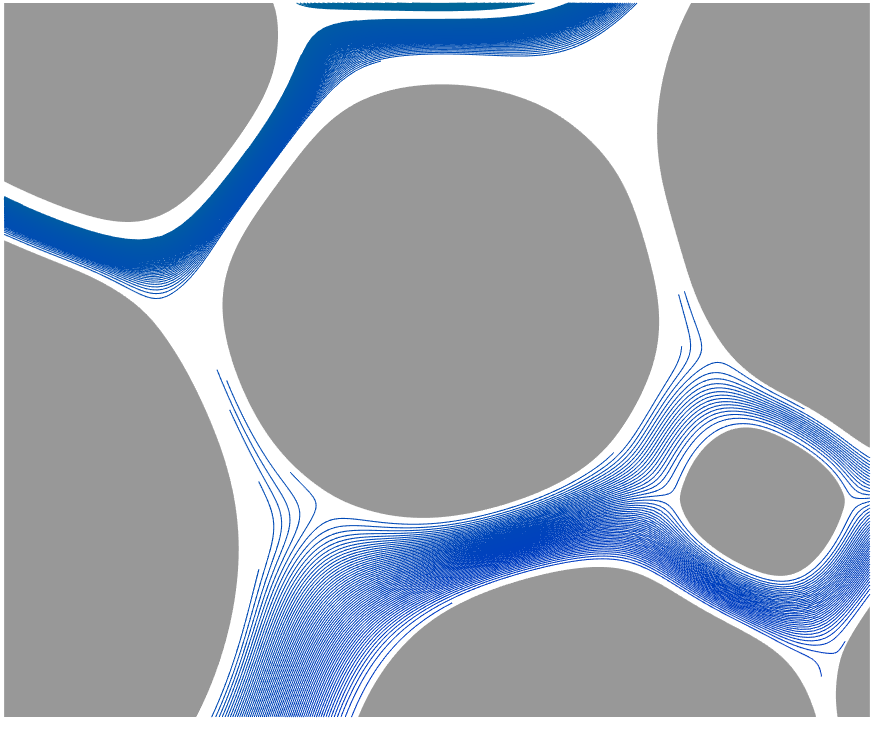
\includegraphics[width = 0.32\textwidth]{./figs/tracer_20b210_zoom}
%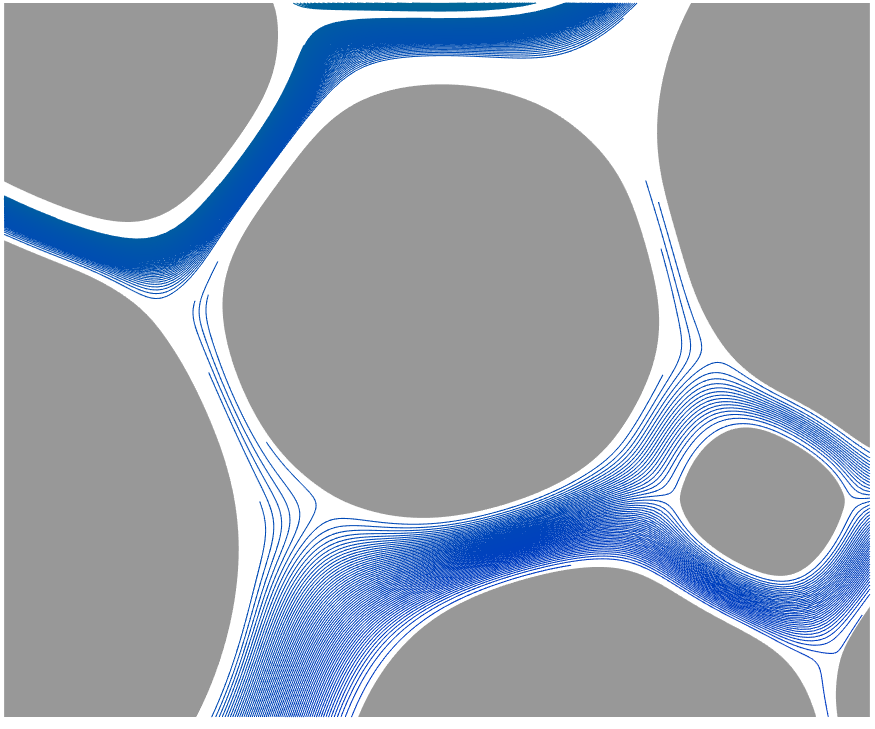
\includegraphics[width = 0.32\textwidth]{./figs/tracer_20b240_zoom}
%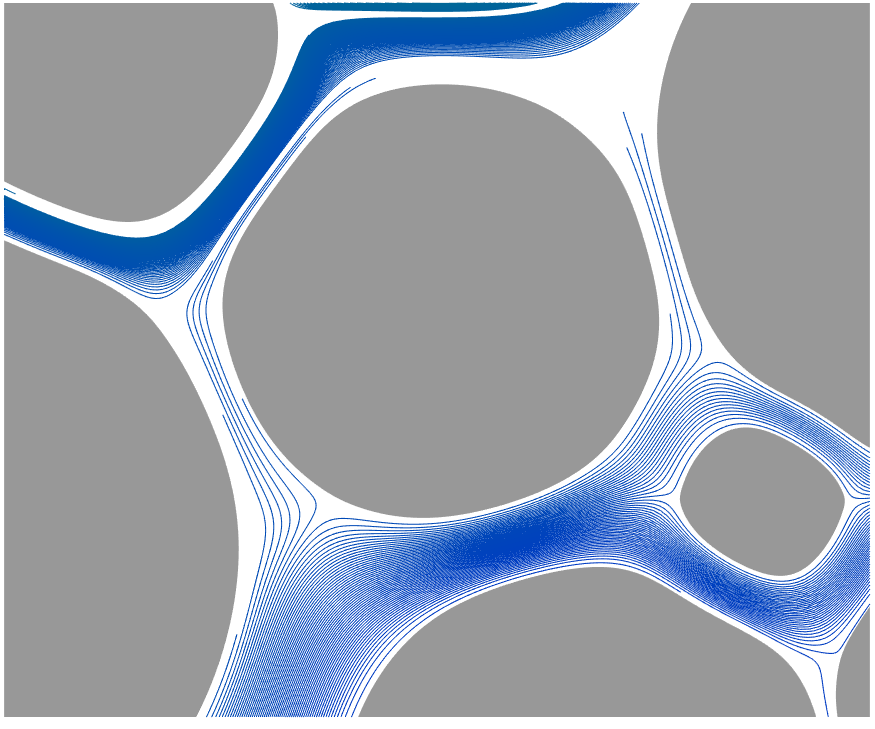
\includegraphics[width = 0.32\textwidth]{./figs/tracer_20b270_zoom}
%\caption{\label{fig:Eroding20zoom}The zoom windows in the last three
%  frames of Figure~\ref{fig:Eroding20tracer}. The trajectories of
%  tracers around the bodies. Since we use a Barycentric quadrature rule
 % and the fourth order Runge Kutta method, the tracers can be very close
 % to but not penetrate the bodies.}
%\end{center}
%\end{figure}
%{\color{red}
%In Fig.~\ref{fig:Eroding20tort} we release 1000 tracers 
%from the starting cross section x = -1 to 
%the end cross section x = 1 and 
%use the local tortuosity to analysis the effect
%of the geometrical structure on fluid velocity field when the porosity is 62.9 \%.
%In Fig.~\ref{fig:Eroding20tort}(a) the graph represents the ratio of the
%x-component velocity u(-1, y) to its maximum velocity $u_{max}=2.9828
%\times 10^{-3}$ at equal spreading tracers on the starting cross section.
%The velocity is continuous along the starting cross section and
%acting as several Poiseuille flows. This velocity graph is different
%from the one in~\cite{matyka2008tortuosity} since we choose our cross
%section to be the beginning of the flow before the fluid touches any
%body. In Fig.~\ref{fig:Eroding20tort}(b) we record the local tortuosity
%$\tau(y)=\lambda(y)/d$
%of the tracers at $y$ on the starting cross section x = -1 
%where $d = 2$.
%This graph is not continuous 
%and the jumps in $\tau$ mean that the initial neighboring tracers have been
%seperated by the bodies. 
%The maximum of $\tau$ is 1.2713 and the minimum is 1.0001.
%}
%{\color{red}
%In Fig.~\ref{fig:Eroding20tort}(c) we calculate the difference of 
%$\tau$ at two neighboring tracers 
%and draw the trajectories of neighboring tracers
%if the difference of $\tau$ at the neighboring tracers is large. 
%From Fig.~\ref{fig:Eroding20tort}(c), we collect the 10 largest difference of $\tau$ 
%at the neighboring tracers and 
%draw the pair of trajectories in the same color and 
%are able to tell the neighboring trajectories will be very 
%different if they are separated by bodies.
%For each pair of trajectories, 
%they are splitted by the body at the left side of the body, then
%one of them goes up and the other one goes down along the body 
%until they rejoin with each other at the right side of body.  
%Furthermore, the pair trajectories could be splitted by more than one body, 
%for example in Fig.~\ref{fig:Eroding20tort}(c) the toppest red pair trajectories 
%are splitted by two close bodies.
%}

%To measure the local behavior of fluid quantitatively, 
%we use the velocities and local tortuosities at the starting cross section 
%to analysis the interaction of fluid and bodies until the end cross section 
%in Fig.~\ref{fig:Eroding100tort}(b) and (c).
%In Fig.~\ref{fig:Eroding100tort}(b) the graph represents the ratio of the
%x-component velocity u(-1, y) to its maximum velocity $u_{max}=3.9021
%\times 10^{-4}$ at equal spreading tracers on the strating cross section.
%As in the case of 20 nearly touching bodies, the velocity is continuous along
%the starting cross section and acting as a Poiseuille flow in the channel between
%bodies. When the fluid is close to bodies
%the speed of fluid will be slow down because of the no-slip condition on the bodies
%and this causes the separated branches of the inlet flow.
%The maximum velocity of the fluid with 100 bodies on the starting cross 
%section is slower than the maximum velocity of the fluid with 20 bodies
%but the velocity in the case of 100 bodies 
%changes more rapidly than the velocity of the fluid with 20 bodies.
%The reason of the rapid change on the starting cross section of 
%100-body case is because there are 
%more bodies near the starting cross section in
%100-body case than in the 20-body case. 
%so the inlet flow in 100-body case
%will be separated into more branches than the flow in 20-body case. 
%
%In Fig.~\ref{fig:Eroding100tort}(c) we record the 
%local tortuosity $\tau(y)$ for $y$ on the starting cross section x = -1.
%It is a discontinous function and the maximum of $\tau$ in the case of 100 bodies
%is 1.2547 and the minimum is 1.0003. This function $\tau$
%has more jumps than the one in the case of 20 bodies but its maximum 
%is smaller than the maximum in the case of 20 bodies. 
%The jump in this graph means the neighboring trajectories are splitted by bodies
%so it is reasonable to have more jumps in the case of 100-body than the case of 20-body
%since there are more bodies in the former case. 

%To study the behavior of fluid in the porous media with multiple bodies, 
%we release 1000 tracers equispaced in $y$ from the 
%cross section x = -1 and record their trajectories and velocities
%until they arrive the end cross section x = 1 
%and the porosity of this geometric structure is 62.98 \%. 
%To understand the global action of fluid qualitatively, 
%we only draw 200 historical trajectories from x = -1 to x = 1 
%in Fig.~\ref{fig:Eroding100tort}(a). 
%When equispaced tracers are released in a 2D tube without any grains, 
%the streamlines are straight 
%and the intersection points of streamlines and any cross section are equispaced. 
%But it is not the same when there are bodies in the fluid. 
%In Fig.~\ref{fig:Eroding100tort}(a)
%even the tracers are equispaced in $y$ on the cross section $S$, 
%the streamlines have been push up and down by the bodies and
%some of them are close together. 
%
%
%%To understand the meaning of jump 
%%of $\tau$, we use the data we got from local tortuosity $\tau(y)$
%%to find the difference of $\tau$ at the neighboring tracers in Fig.~\ref{fig:Eroding100tort}(c) 
%%and draw 50 pairs of neighboring trajectories which have the largest difference of $\tau$
%%in Fig.~\ref{fig:Eroding100tort_traj}. These pairs of two neighboring trajectories are splitted by bodies
%%then rejoin with each other and the splitting-rejoining behavior causes the difference of $\tau$ with respect to the neighboring trajectories.   
%%We also can get the idea why the maximum value of $\tau$ is smaller 
%%than the one in the case of 20 bodies . 
%%The most of the bodies in this case are smaller than those in the case of 20 bodies.
%%So when two neighboring trajectories are splitted on the left side by a smaller body they do not
%%travel as far as the two splitted by a bigger body do after they rejoin on the right side. 


%{\color{red}
%This case is 100 bodies in a Hagen-Poiseuille flow. The background
%flow is 
%\begin{align}
%  \UU(\xx)=U \left[
%  \begin{array}{c}
%    1-y^2 \\ 0
%  \end{array}
%  \right]
%\end{align}
%with floating flow rate $U$ such that pressure drop is fixed from x = -2 to x = 2.
%We record the vorticity of 
%fluid in colormap during the bodies erosion in Fig.~\ref{fig:Eroding100vort} and 
%measure the gap sizes between bodies in Fig.~\ref{fig:Eroding100gap} at four equispaced times.
%Since the vorticity is equivalent to the shear stress and the erosion is faster in the regions where
%the magnitude of the vorticity is larger 
%so the erosion is getting faster and faster 
%from the first snapshot to the forth one in Fig.~\ref{fig:Eroding100vort}.
%At t = 0.005 the porosity is 55.54\% and the most gap sizes between bodies are less than 0.015 in 
%Fig.~\ref{fig:Eroding100gap}(a). Since some of the bodies are vanished in the fluid, the numner of gaps 
%decreases and the gap sizes get larger and larger between the remaining bodies. 
%In Fig.~\ref{fig:Eroding100gap}(b) and (c) we still can see small gap sizes are in the majority but 
%it is not as concentrated as the one we see in Fig.~\ref{fig:Eroding100gap}(a). 
%In Fig.~\ref{fig:Eroding100gap}(d) there are only 254 gaps between 82 bodies and 
%the distribution of gap sizes spreads over without any major pack.  
%}
%



\end{document}


